\documentclass[a4paper]{article}
\usepackage[T1]{fontenc}			% pacchetto per \chapter
\usepackage[italian]{babel}
\usepackage[italian]{isodate}  		% formato delle date in italiano
\usepackage{graphicx}				% gestione delle immagini
\usepackage{amsfonts}
\usepackage{booktabs}				% tabelle di qualità superiore
\usepackage{amsmath}				% pacchetto matematica
\usepackage{mathtools}				% per sottolineare sotto le equazioni
\usepackage{stmaryrd} 				% per '\llbracket' e '\rrbracket'
\usepackage{amsthm}					% teoremi migliorati
\usepackage{enumitem}				% gestione delle liste
\usepackage{pifont}					% pacchetto con elenchi carini
\usepackage{enumitem}				% pacchetto per elenchi con lettere dell'alfabeto
\usepackage{cancel}					% per cancellare delle espressioni matematiche
\usepackage{caption}				% caption personalizzati
\usepackage[]{mdframed}				% box per il testo
\usepackage{multirow}				% più linee in una tabella
\usepackage{gensymb}				% simbolo di degree


% draw a frame around given text
\newcommand{\framedtext}[1]{%
	\par%
	\noindent\fbox{%
		\parbox{\dimexpr\linewidth-2\fboxsep-2\fboxrule}{#1}%
	}%
}



\usepackage[x11names]{xcolor}		% pacchetto colori RGB
% Link ipertestuali per l'indice
\usepackage{xcolor}
\usepackage[linkcolor=black, citecolor=blue, urlcolor=cyan]{hyperref}
\hypersetup{
	colorlinks=true
}

\usepackage{tikz}
\newcommand{\MyTikzmark}[2]{%
	\tikz[overlay,remember picture,baseline] \node [anchor=base] (#1) {#2};%
}
\newcommand{\DrawVLine}[3][]{%
	\begin{tikzpicture}[overlay,remember picture]
		\draw[shorten <=0.3ex, #1] (#2.north) -- (#3.south);
	\end{tikzpicture}
}
\newcommand{\DrawHLine}[3][]{%
	\begin{tikzpicture}[overlay,remember picture]
		\draw[shorten <=0.2em, #1] (#2.west) -- (#3.east);
	\end{tikzpicture}
}


%\usepackage{showframe}				% visualizzazione bordi
%\usepackage{showkeys}				% visualizzazione etichetta

\newtheorem{theorem}{\textcolor{Red3}{\underline{Teorema}}}
\newtheorem{lemma}{Lemma}
\renewcommand{\qedsymbol}{QED}
\newcommand{\exec}[1]{\llbracket #1\:\rrbracket}
\newcommand{\dquotes}[1]{``#1''}
\newcommand{\longline}{\noindent\rule{\textwidth}{0.4pt}}
\newcommand{\circledtext}[1]{\raisebox{.5pt}{\textcircled{\raisebox{-.9pt}{#1}}}}

\newenvironment{rowequmat}[1]{\left(\array{@{}#1@{}}}{\endarray\right)}
\newenvironment{rowequmatbra}[1]{\left[\array{@{}#1@{}}}{\endarray\right]}

\begin{document}
	\author{VR443470}
	\title{Schemi Analisi II}
	\date{\printdayoff\today}
	\maketitle
	
	\newpage
	
	% indice
	\tableofcontents
	
	\newpage
	
	\section{Prerequisiti}\label{section: prerequisiti}
	
	Il corso di Analisi II si articola in due macro sezioni: primo e secondo parziale. All'esame gli esercizi da svolgere saranno 10, suddivisi 5 per la prima parte e 5 per la seconda.\newline
	
	\noindent
	Nonostante vengano date 3 ore per svolgere l'esame totale, dunque 1 ora e mezza per ciascuna prova parziale, il tempo è una risorsa fondamentale. Difatti, se un calcolo matematico dovesse richiedere una quantità eccessiva di risorse/tempo, si rischierebbe di non passare l'esame con esito positivo.\newline
	
	\noindent
	Risulta dunque fondamentale, per ciascun studente, giungere con dei prerequisiti solidi e non banali. In questo capitolo si provvederà a fornire alcuni prerequisiti necessari per affrontare il percorso senza eccessive difficoltà.\newline
	
	\noindent
	Ogni paragrafo presenterà degli esercizi e ognuno di essi sarà risolto nel seguente modo: il primo in modo approfondito per illustrare il modus operandi, gli altri facendo vedere i calcoli e risparmiando le spiegazioni prolisse. Chiaramente, nel caso in cui ci dovesse essere un caso particolare, esso verrà affrontato e spiegato passo passo.\newpage
	
	\subsection{Geometria analitica}\label{subsection: geometria analitica}
	
	\subsubsection{Circonferenza}\label{subsubsection: circonferenza}
	
	La circonferenza è graficamente rappresentata nel seguente modo:
	\begin{figure}[!htp]
		\centering
		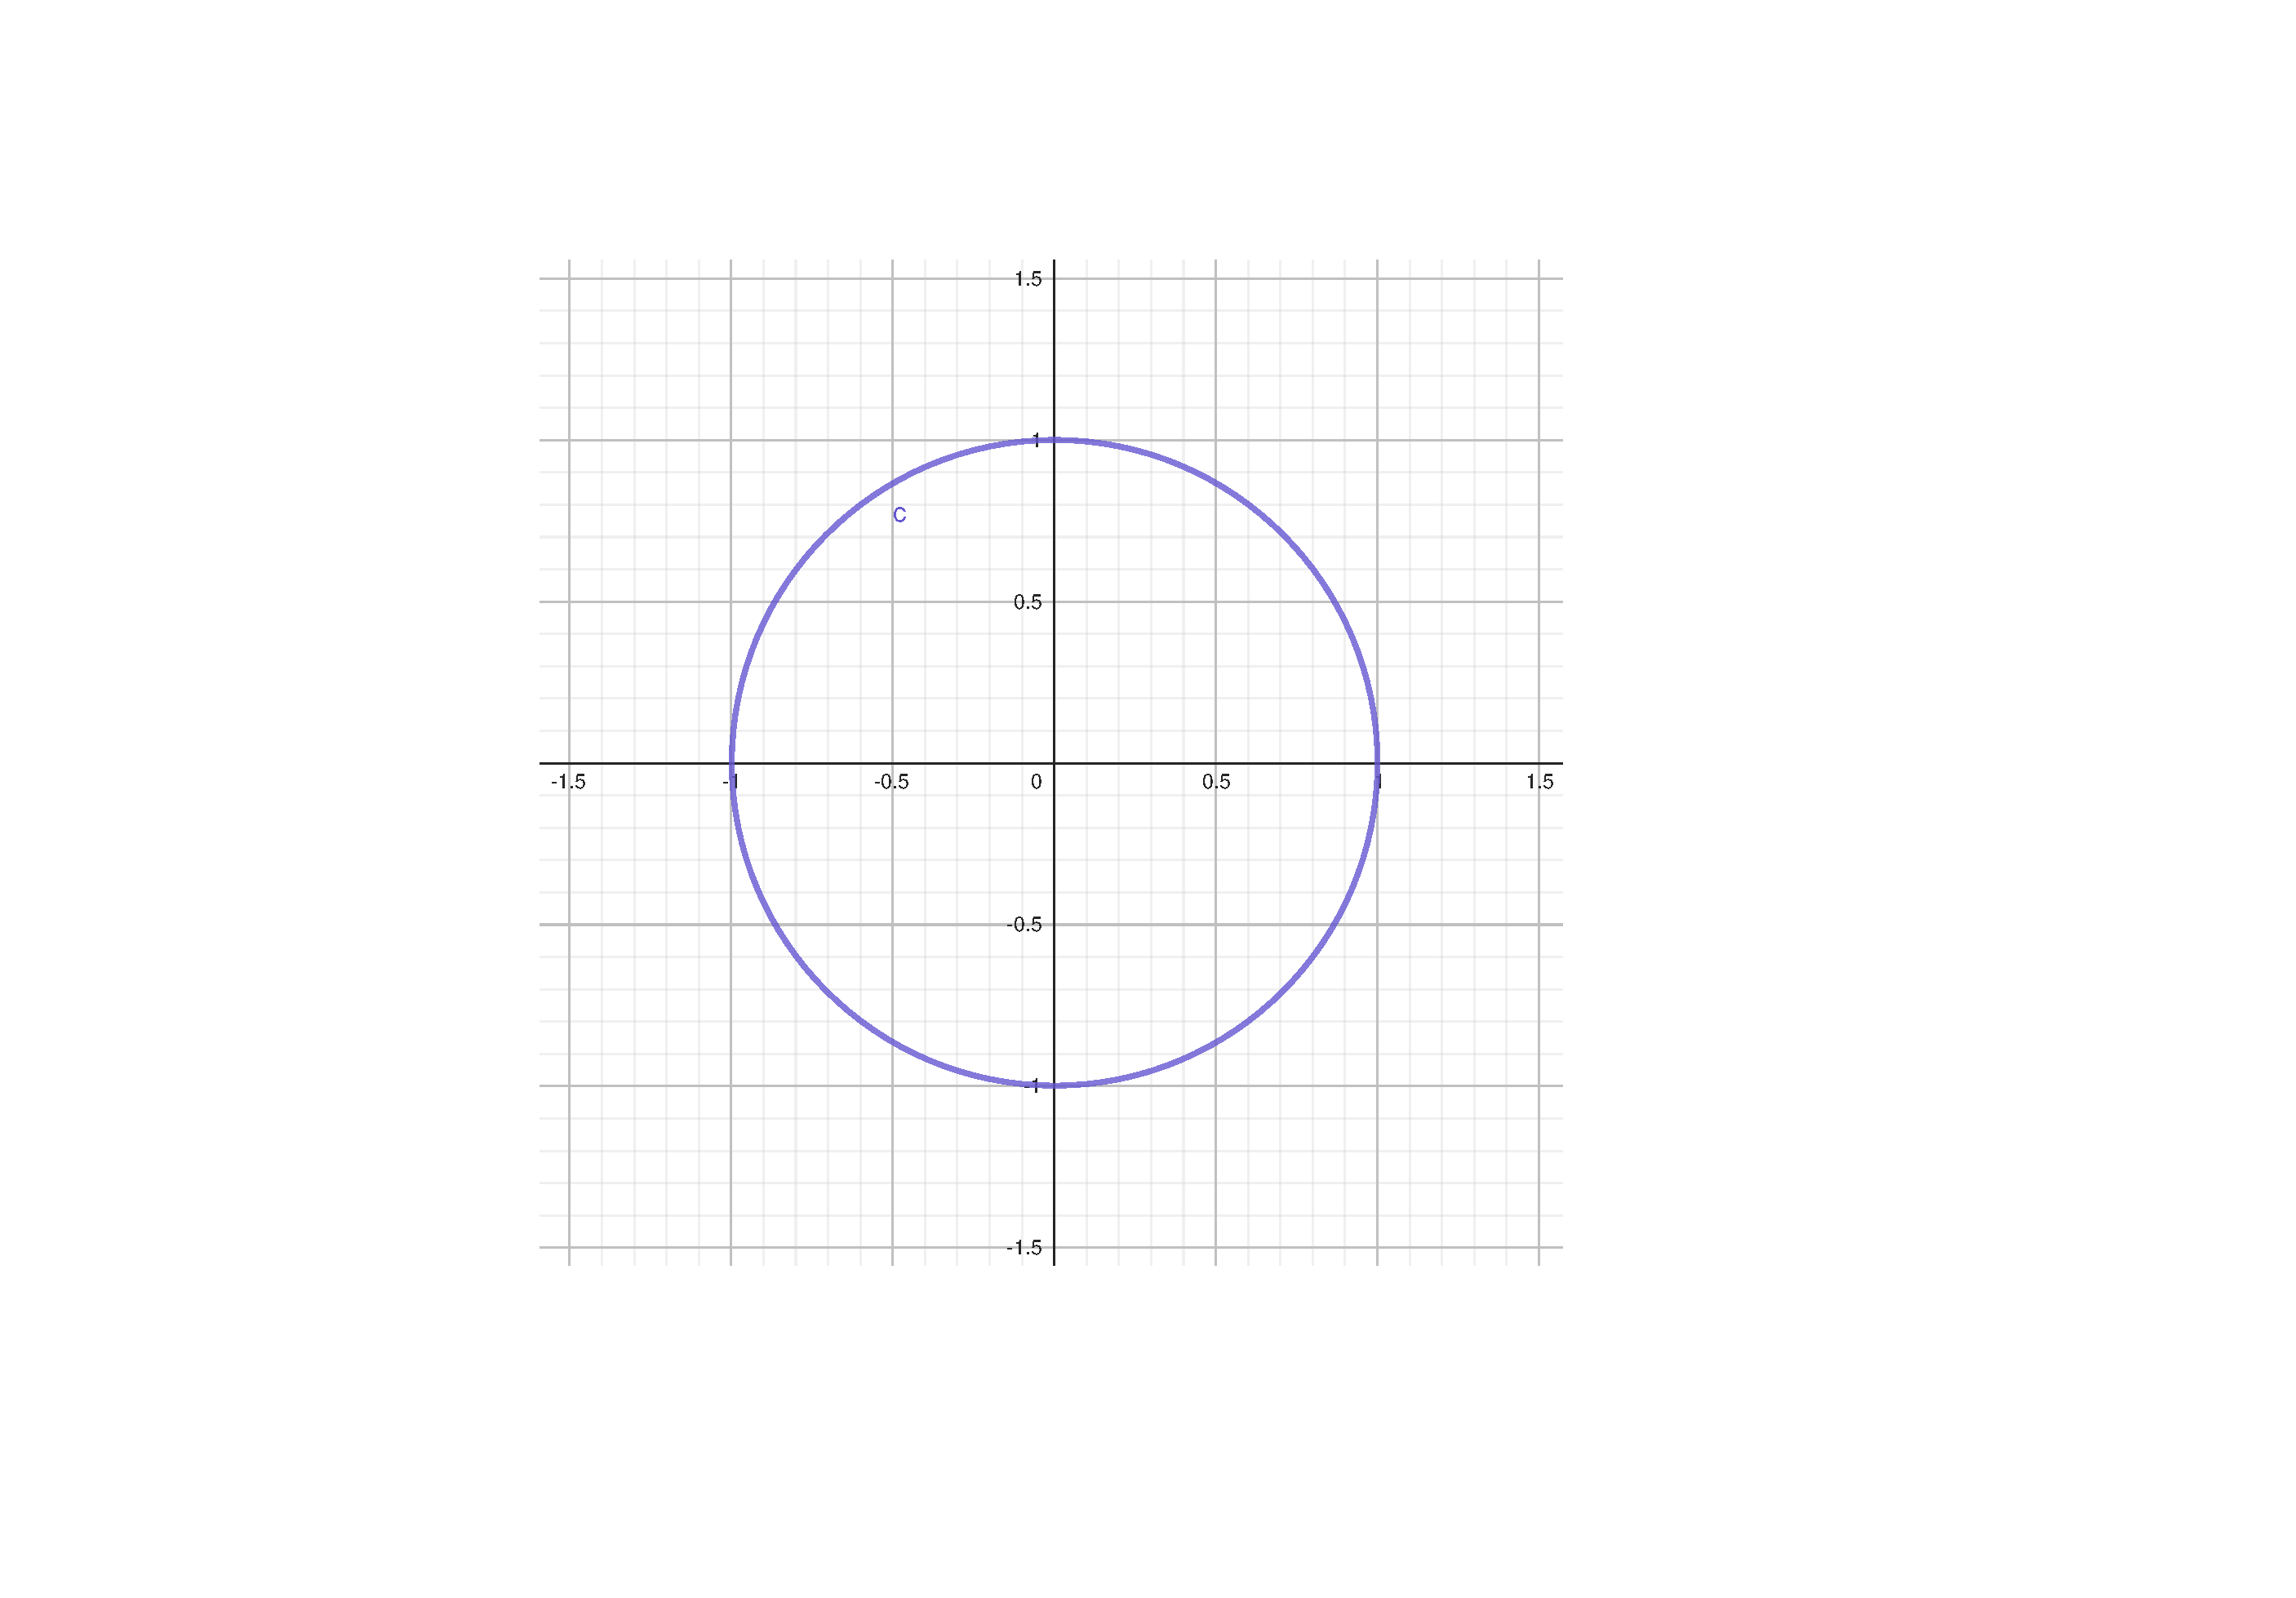
\includegraphics[width=.6\textwidth]{img/circonferenza.pdf}
	\end{figure}
	
	\noindent
	Chiamando con $C = \left(x_{C}, y_{C}\right)$ le coordinate del centro della circonferenza e con $r$ il raggio, la sua equazione generale è espressa nel seguente modo:
	\begin{equation*}
		\left(x-x_{C}\right)^{2} + \left(y-y_{C}\right)^{2} = r^{2}
	\end{equation*}
	Nel caso in cui la circonferenza fosse centrata nell'origine degli assi, ovvero $C = \left(0,0\right)$, allora l'equazione generale sarebbe ridotta a:
	\begin{equation*}
		x^{2} + y^{2} = r^{2}
	\end{equation*}
	Per essere più precisi, l'\textbf{equazione canonica} corrispondente alla circonferenza è la seguente:
	\begin{equation*}
		x^{2} + y^{2} + \alpha x + \beta y + \gamma = 0
	\end{equation*}
	Le formule più importanti per ricavare il centro della circonferenza $C$ e il raggio $r$:
	\begin{equation*}
		C = \left(-\dfrac{\alpha}{2}, -\dfrac{\beta}{2}\right) \hspace{1em} ; \hspace{1em} r = \sqrt{\dfrac{\alpha^{2}}{4} + \dfrac{\beta^{2}}{4} - \gamma}
	\end{equation*}
	Per ottenere l'equazione generale partendo dall'equazione canonica, si utilizza il metodo dei completamento dei quadrati (paragrafo~\ref{subsubsection: completamento dei quadrati}).\newline
	
	\noindent
	Per ottenere il raggio nel caso in cui sia noto il centro $C$ e un punto $P = \left(x_{P}, y_{P}\right)$ appartenente alla circonferenza, si utilizza la seguente formula:
	\begin{equation*}
		r = \sqrt{\left(x_{P} - x_{C}\right)^{2} + \left(y_{P} - y_{C}\right)^{2}}
	\end{equation*}
	Per altri approfondimenti: \href{https://www.youmath.it/formulari/formulari-di-geometria-analitica/440-circonferenza-e-cerchio-nel-piano-cartesiano.html}{YouMath}.\newpage
	
	\subsubsection{Ellisse}\label{subsubsection: ellisse}
	
	Non esiste un'unica rappresentazione dell'ellisse, ma solitamente può essere facilmente riconoscibile perché di forma allungata:
	\begin{figure}[!htp]
		\centering
		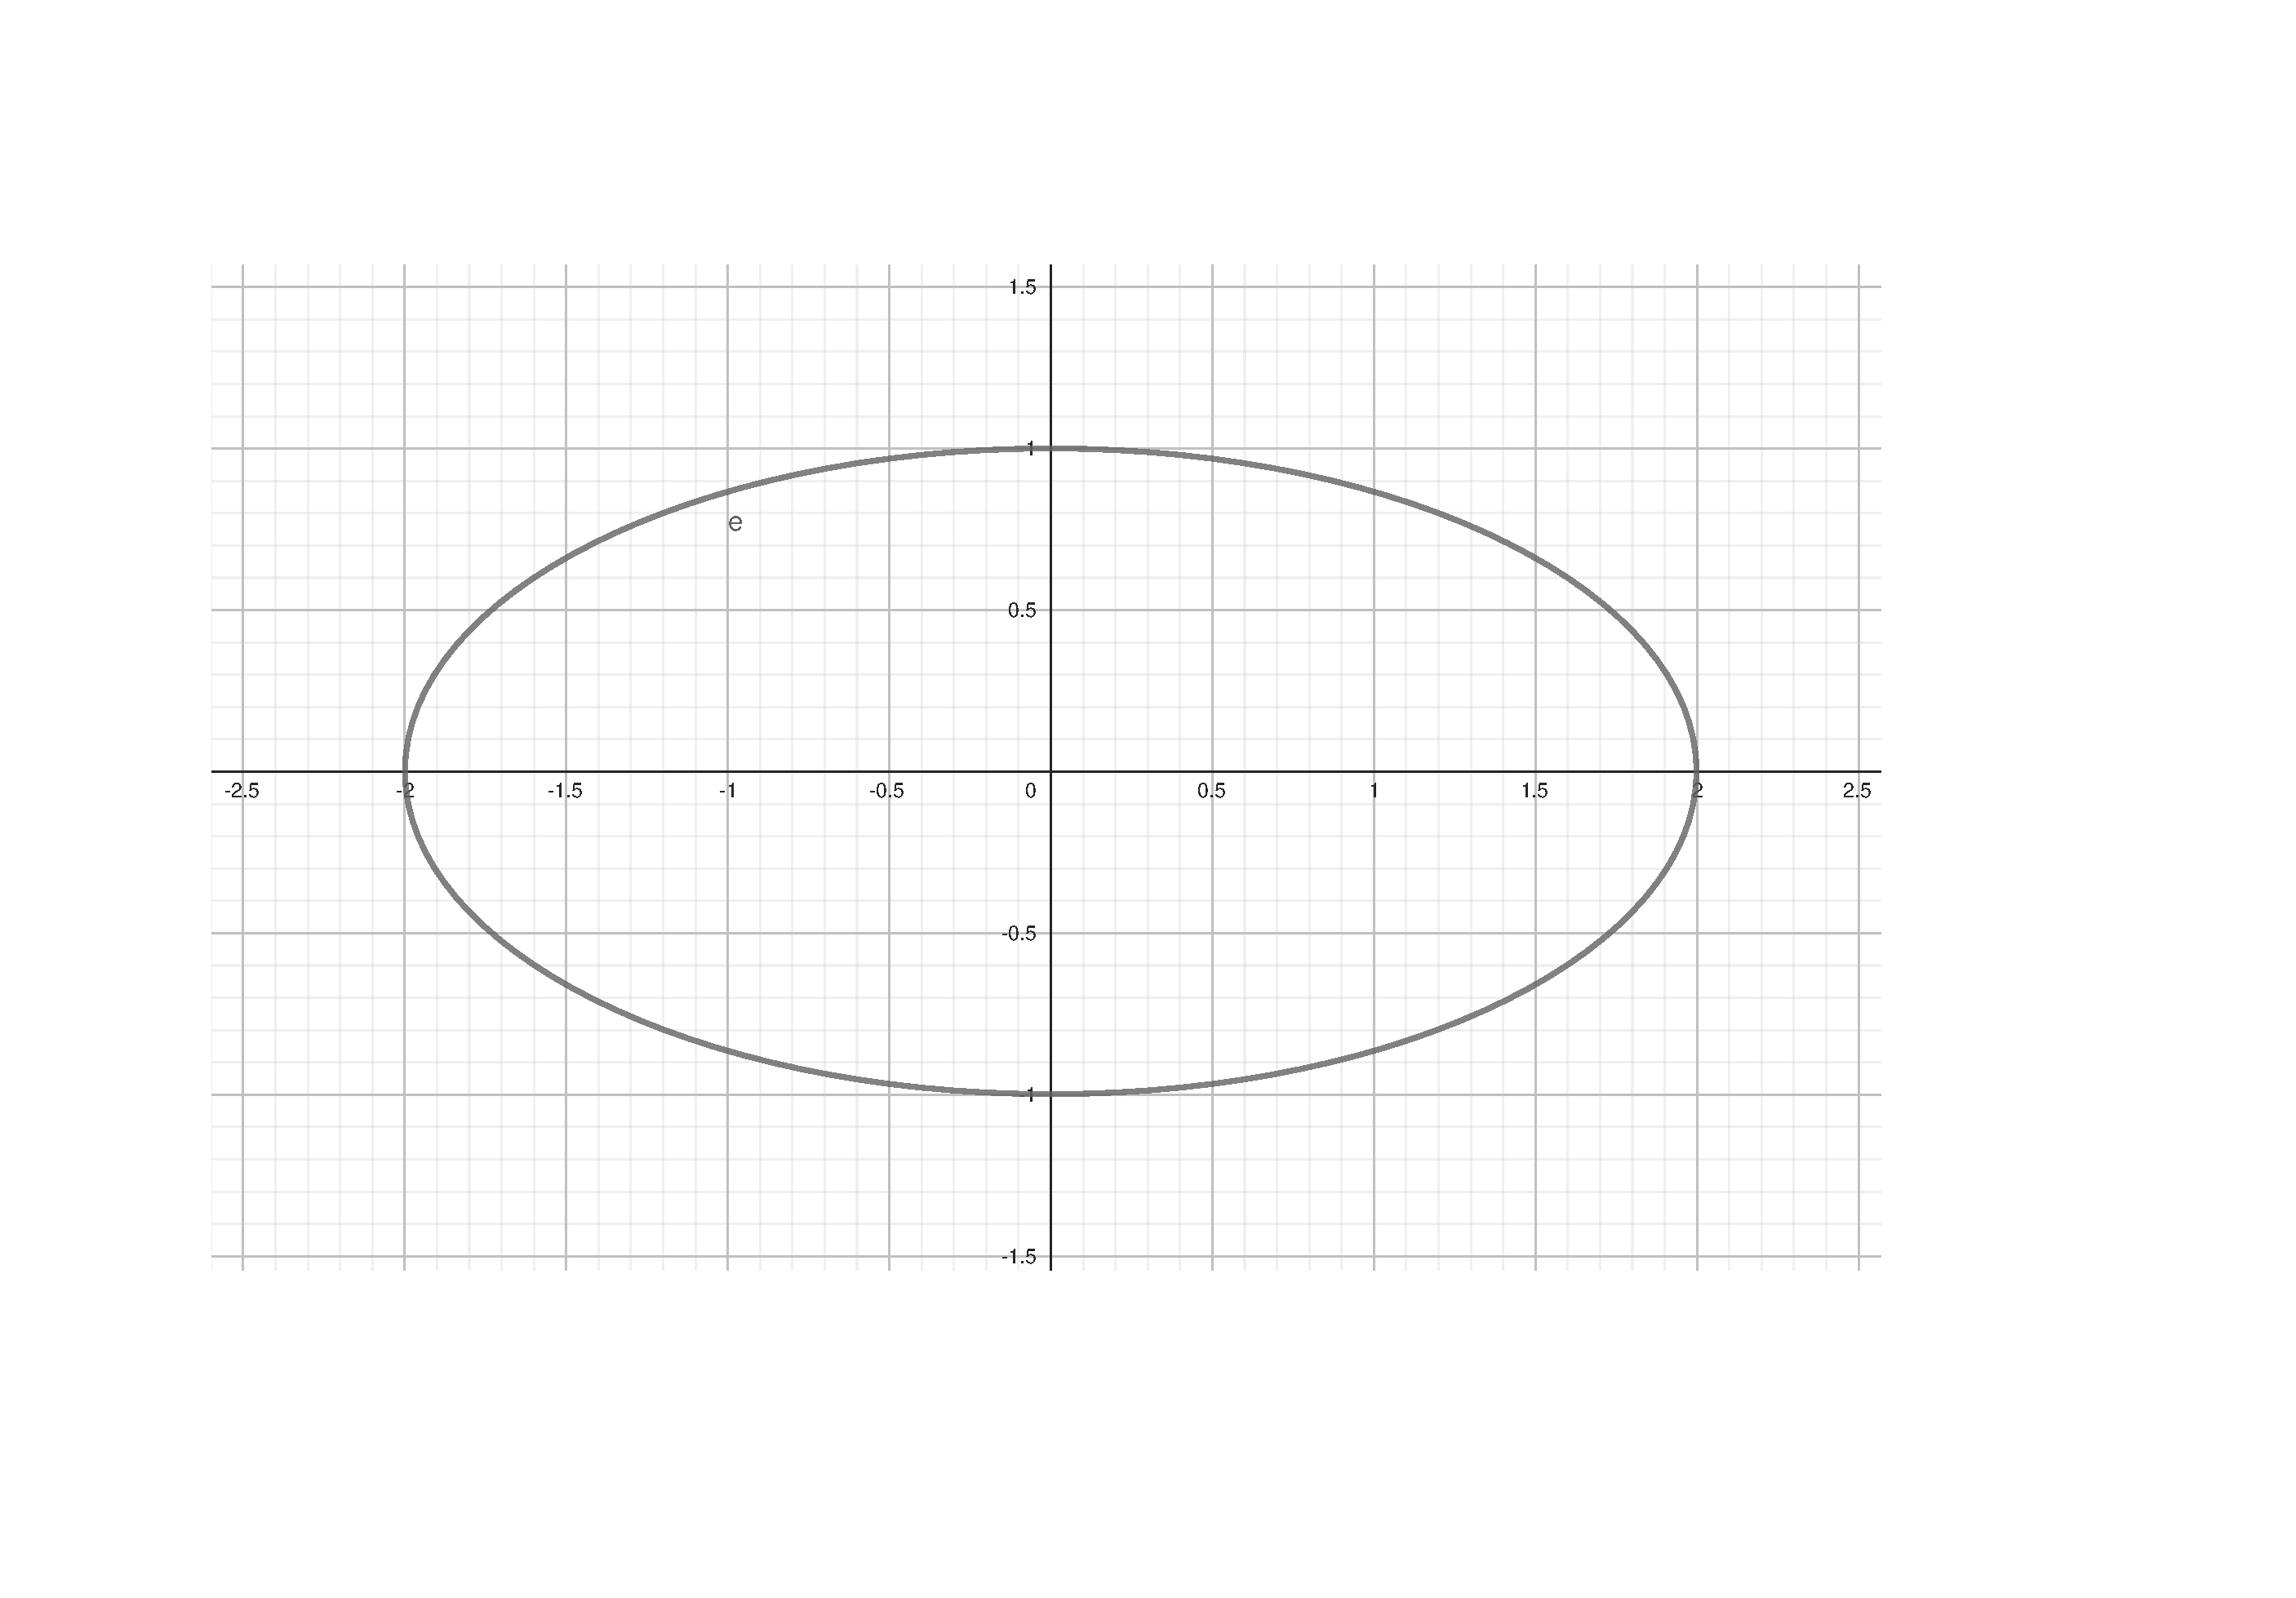
\includegraphics[width=.6\textwidth]{img/ellisse.pdf}
	\end{figure}
	
	\noindent
	Attenzione, che data l'\textbf{equazione canonica} dell'ellisse \textbf{centrata nell'origine}:
	\begin{equation*}
		\dfrac{x^{2}}{a^{2}} + \dfrac{y^{2}}{b^{2}} = 1 \hspace{2em} a \ne 0, \:\: b \ne 0
	\end{equation*}
	Il grafico corrisponde esattamente ad una circonferenza.\newline
	
	\noindent
	Un'ellisse presenta quattro vertici nel caso in cui abbia centro nell'origine. Le relative coordinate sono:
	\begin{equation*}
		V_{1,2} = \left(\pm a, 0\right) \hspace{1em} V_{3,4} = \left(0, \pm b\right)
	\end{equation*}
	Per calcolare l'eccentricità di un'ellisse (\dquotes{quanto l'ellisse è schiacciata}) si devono confrontare i due valori $a^{2}$ e $b^{2}$:
	\begin{equation*}
		\begin{array}{rclcl}
			e = \dfrac{c}{a} & \text{se} & a^{2} > b^{2} & \text{e quindi} & c = \sqrt{a^{2} - b^{2}}\\ [1em]
			e = \dfrac{c}{b} & \text{se} & b^{2} > a^{2} & \text{e quindi} & c = \sqrt{b^{2} - a^{2}}
		\end{array}
	\end{equation*}
	Il valore è compreso tra: $0 \le e < 1$.\newline
	
	\noindent
	Nel caso in cui non fosse centrata nell'origine, l'\textbf{equazione canonica} di un'\textbf{ellisse traslata}, con $C=\left(x_{C}, y_{C}\right)$ come coordinate del centro:
	\begin{equation*}
		\dfrac{\left(x-x_{C}\right)^{2}}{a^{2}} + \dfrac{\left(y-y_{C}\right)^{2}}{b^{2}} = 1
	\end{equation*}
	I relativi vertici hanno le seguenti coordinate:
	\begin{equation*}
		\begin{array}{lcl}
			V_{1} = \left(x_{C}-a, y_{C}\right) &;& V_{2} = \left(x_{C}+a, y_{C}\right) \\
			V_{3} = \left(x_{C}, y_{C}-b\right) &;& V_{4} = \left(x_{C}, y_{C}+b\right) \\
		\end{array}
	\end{equation*}
	L'\textbf{importanza dei vertici} è dovuta al fatto che se fosse necessario rappresentare l'ellisse su un piano cartesiano, grazie alle precedenti formule. È possibile ricordarsi facilmente le formule ricordando che le coordinate dei vertici sono ottenute eseguendo la somma/differenza prima sulla coordinata $x$ e poi sulla coordinata $y$.\newline
	
	\noindent
	Per altri approfondimenti: \href{https://www.youmath.it/formulari/formulari-di-geometria-analitica/445-ellisse-nel-piano-cartesiano.html}{YouMath}.\newpage

	\subsubsection{Iperbole}\label{subsubsection: iperbole}

	Un iperbole con centro nell'origine ha un'equazione del tipo:
	\begin{equation*}
		\dfrac{x^{2}}{a^{2}} - \dfrac{y^{2}}{b^{2}} = \pm 1 \hspace{1.5em} \text{con } a \ne 0, \: b \ne 0
	\end{equation*}
	Il segno $+$ accanto all'$1$ rappresenta l'intersezione con l'asse delle ascisse ($x$), mentre il segno $-$ rappresenta l'intersezione con l'asse delle ordinate ($y$). Graficamente viene rappresentata nel seguente modo:\newline

	\begin{minipage}{.6\textwidth}
		\centering
		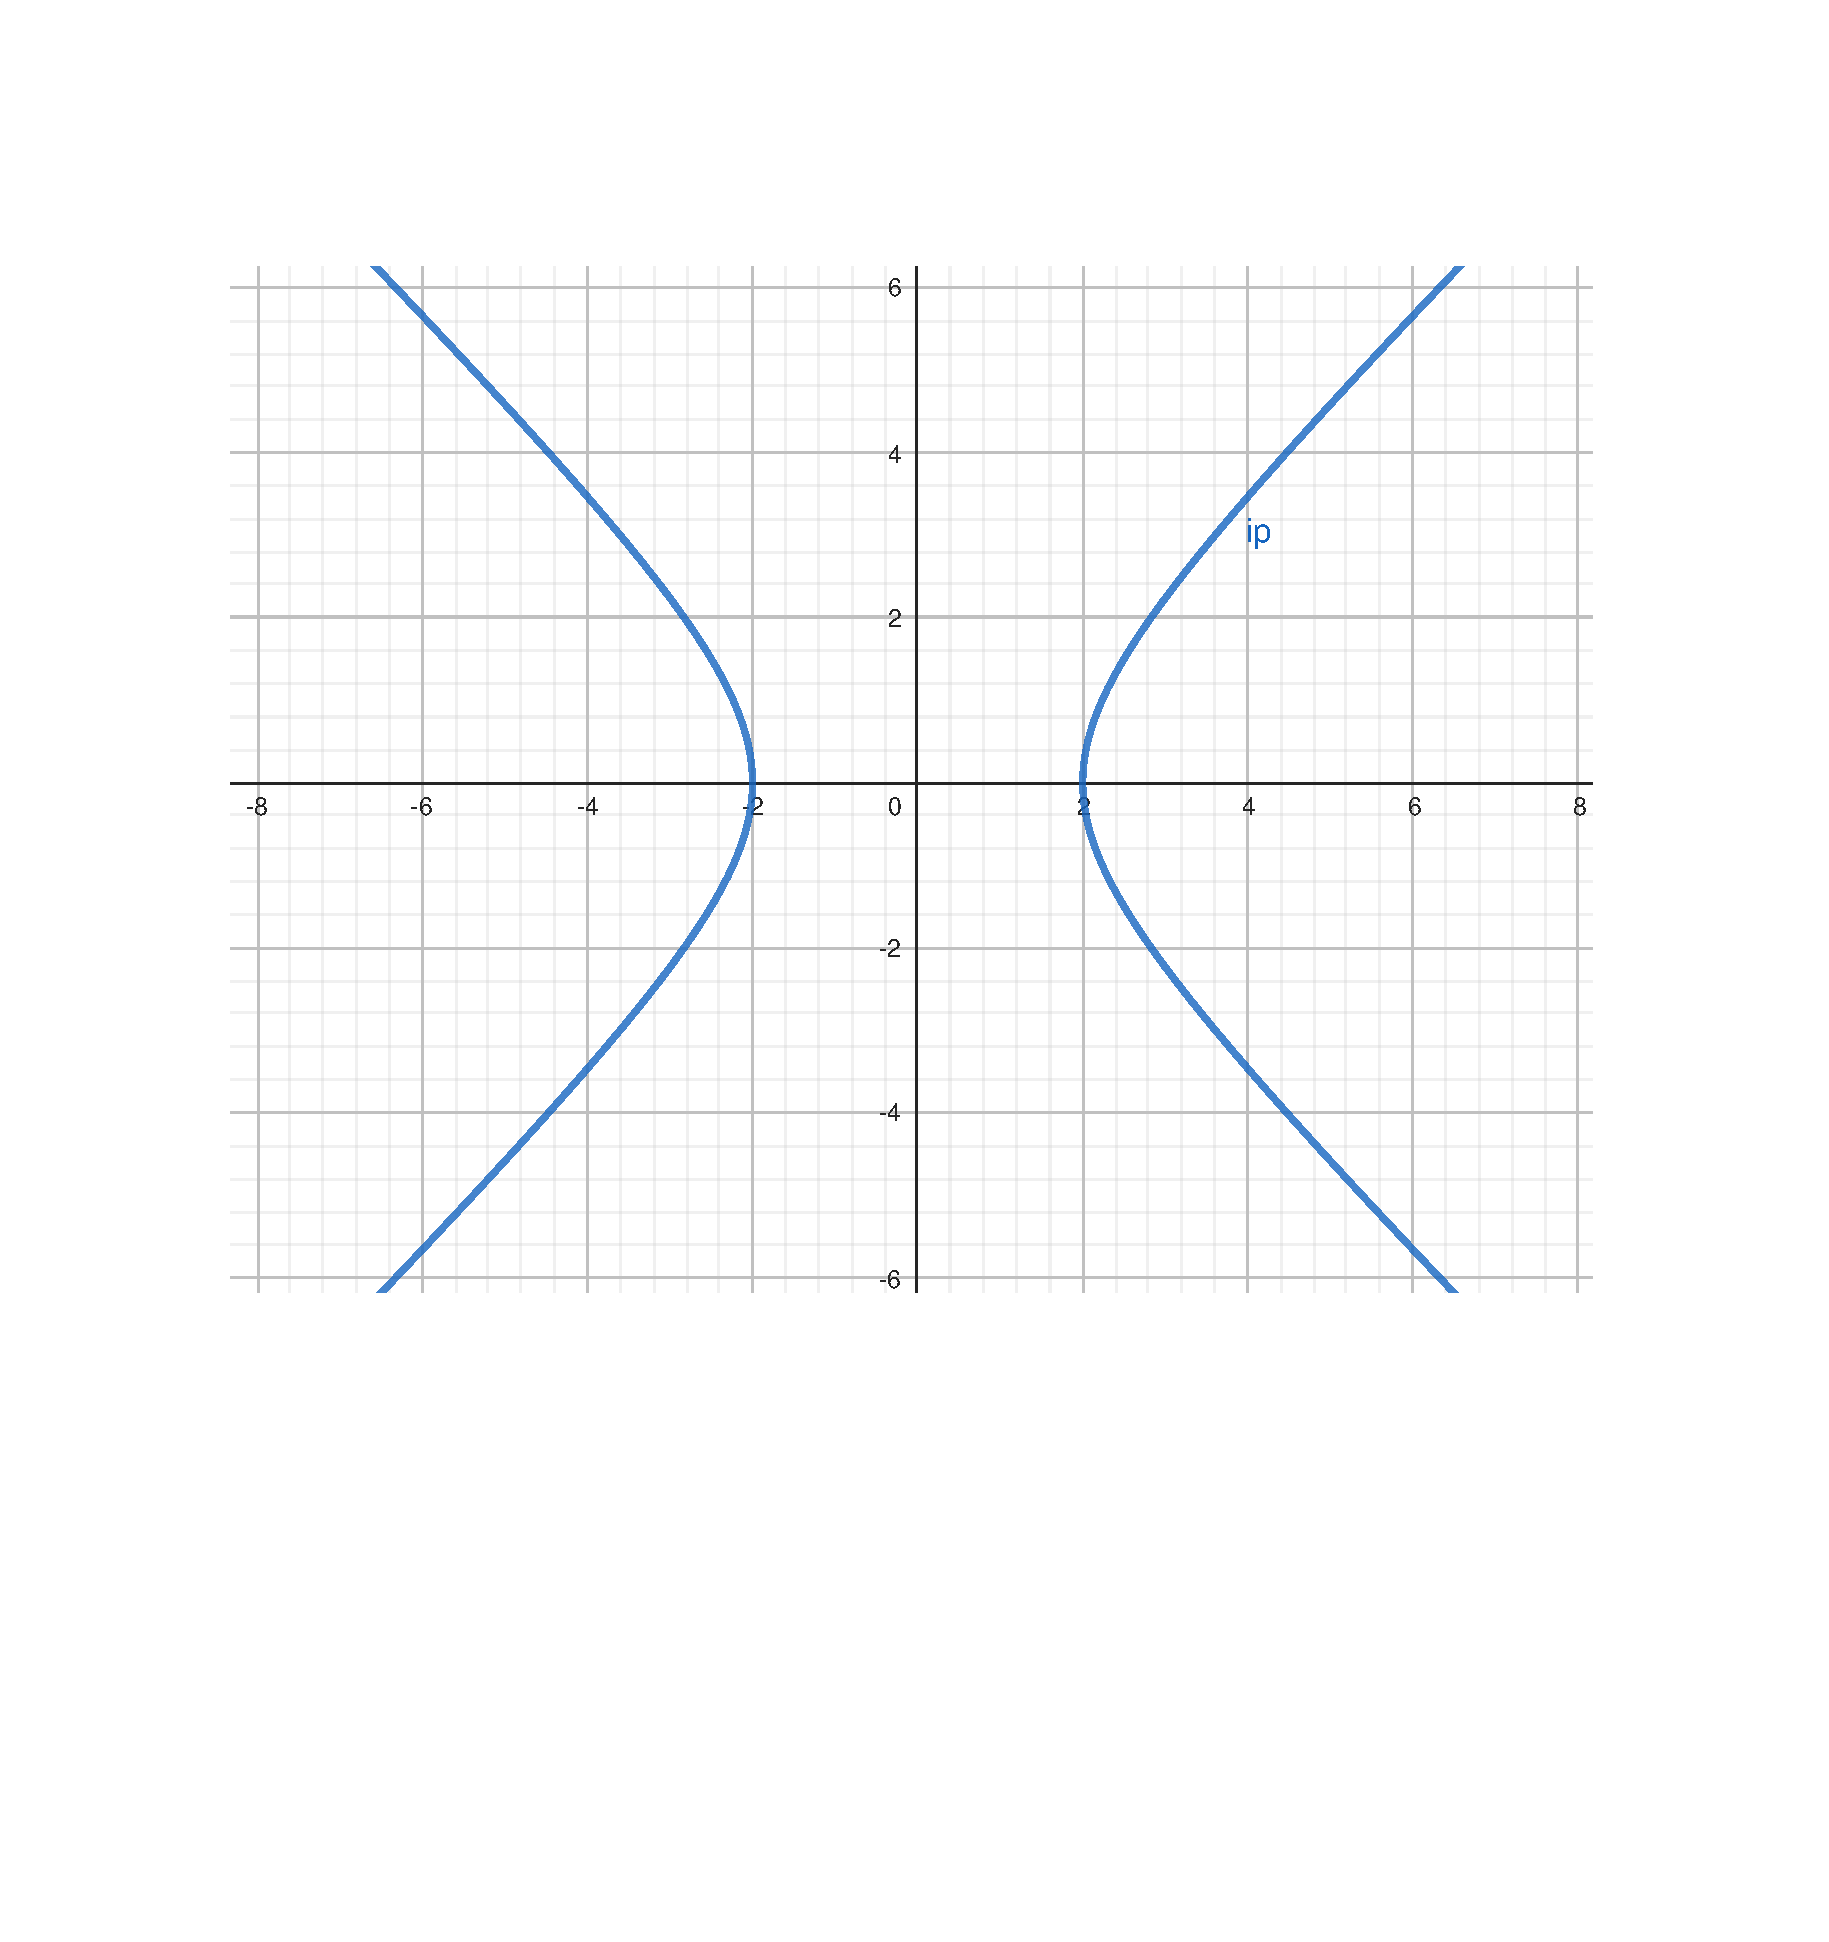
\includegraphics[width=\textwidth]{img/iperbole_ascisse.pdf}
		
		\noindent
		Con $+1$.
	\end{minipage}
	\begin{minipage}{.4\textwidth}
		\centering
		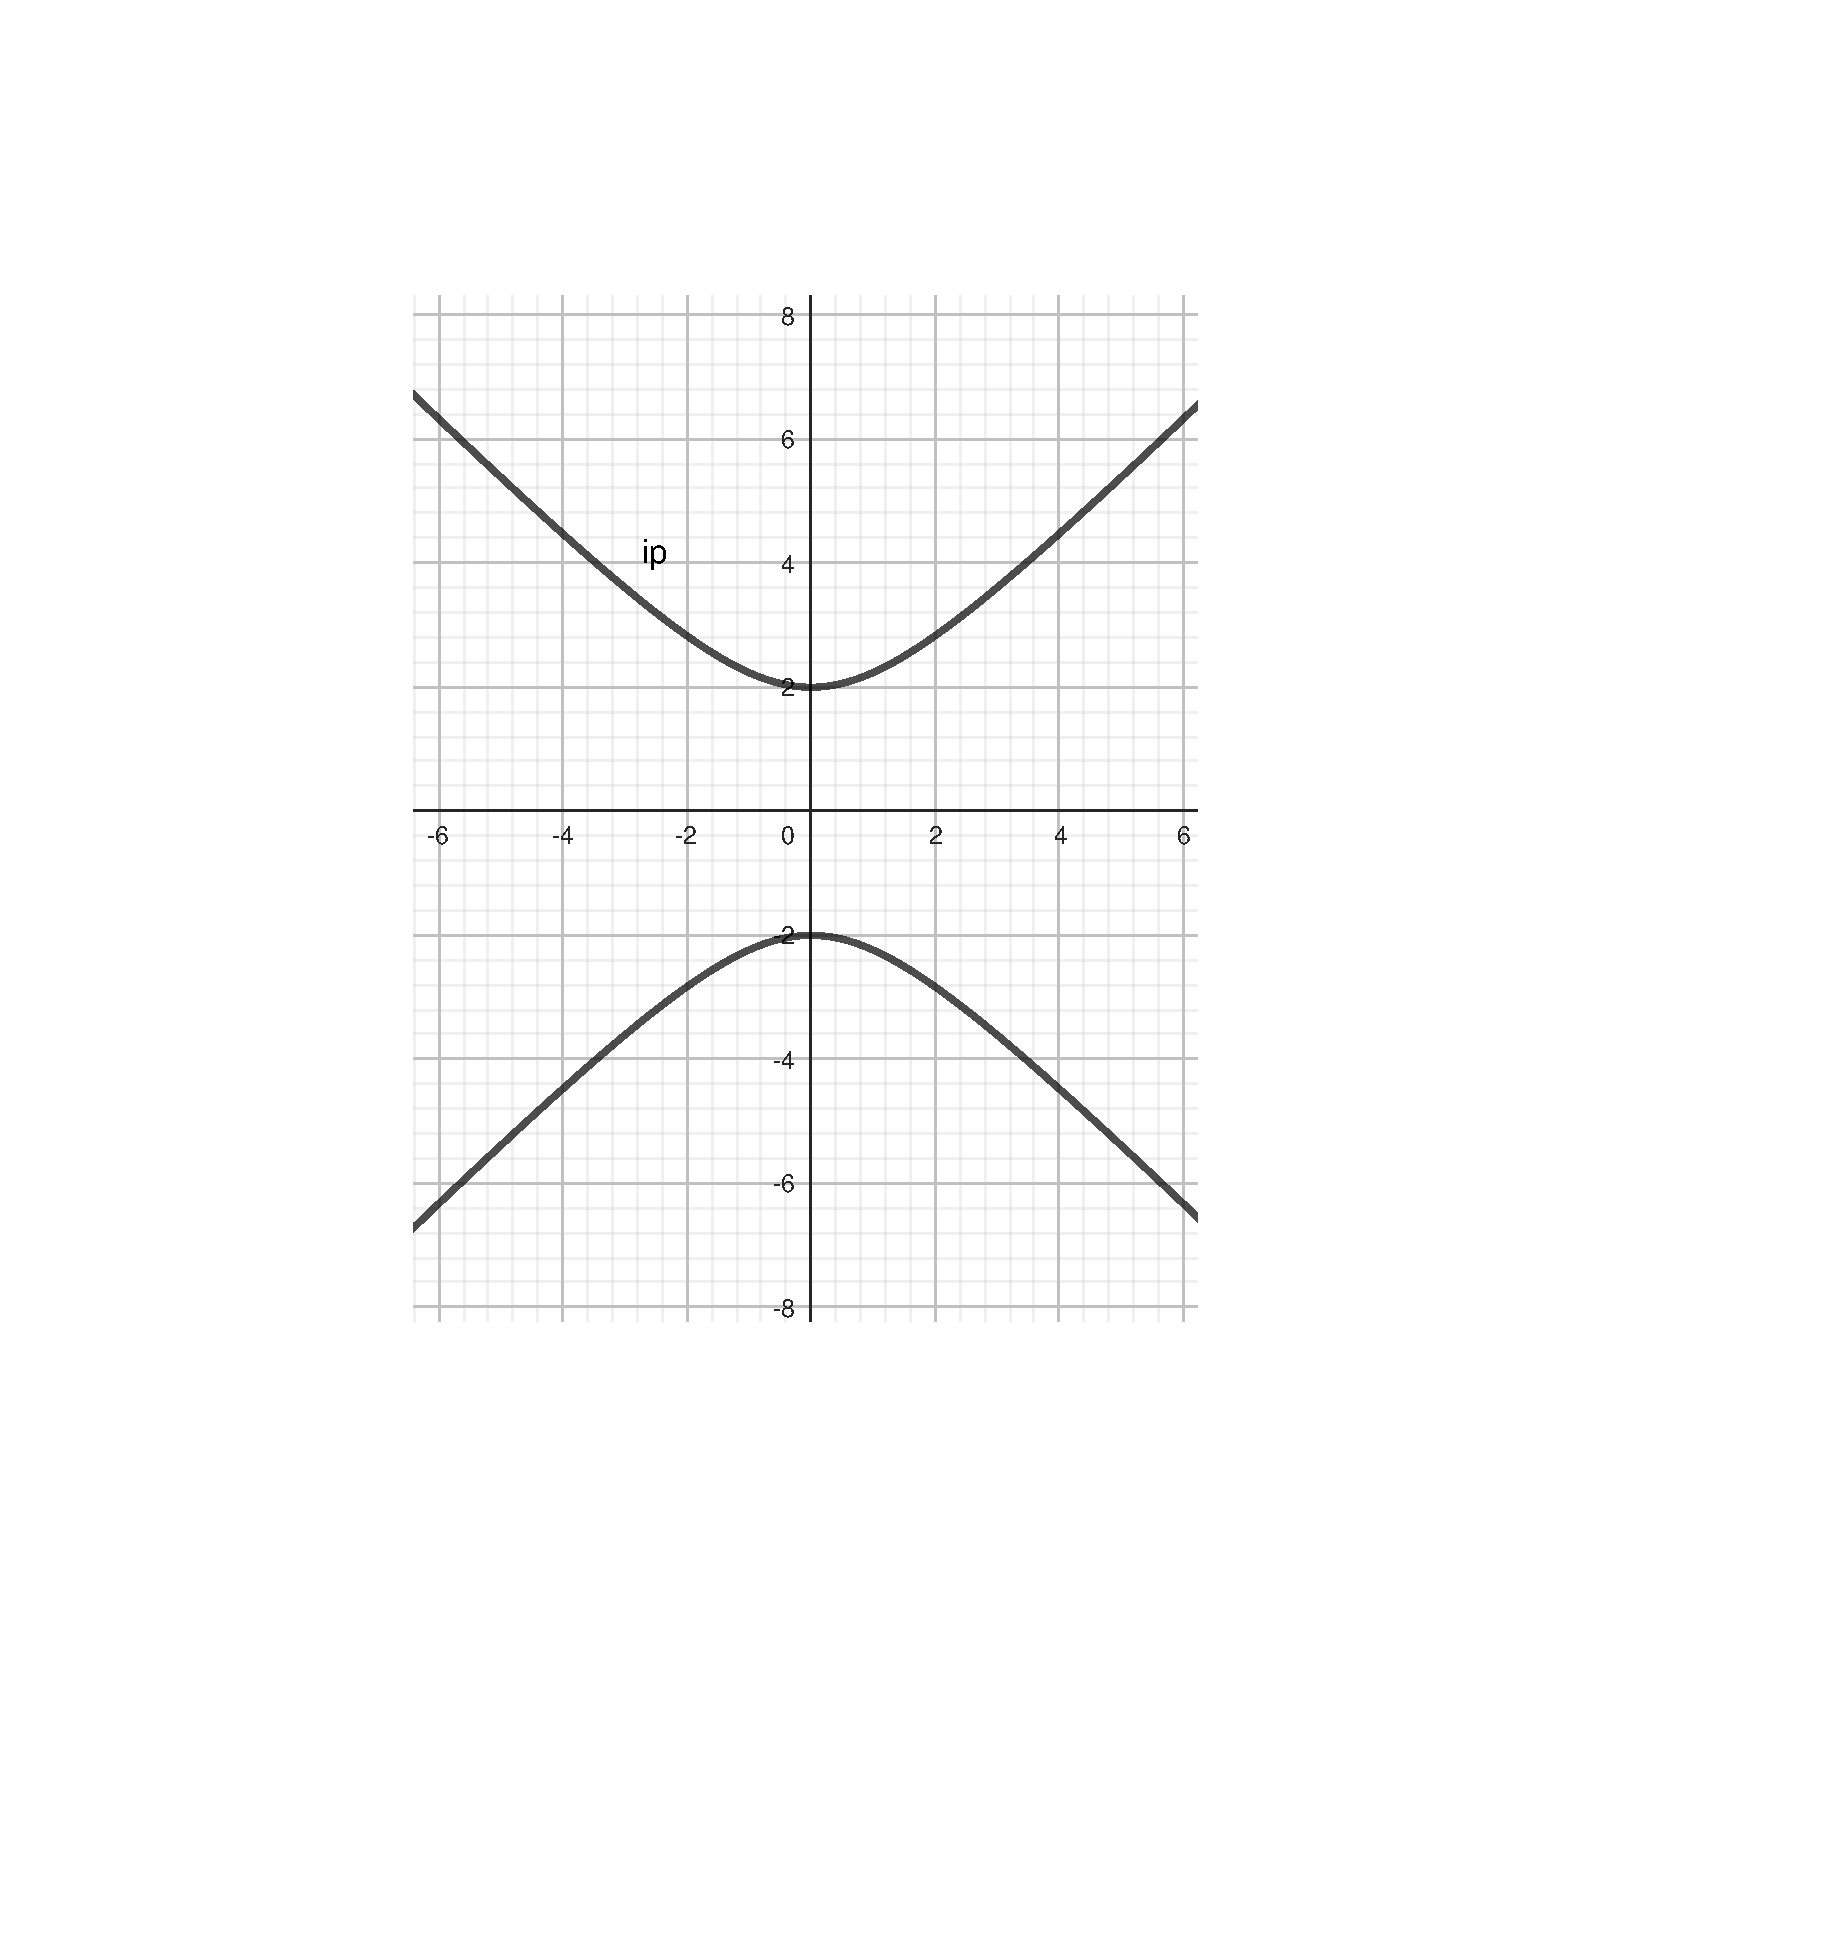
\includegraphics[width=.9\textwidth]{img/iperbole_ordinate.pdf}
		
		\noindent
		Con $-1$.
	\end{minipage}\newline

	\noindent
	Nel caso di una iperbole con gli assi paralleli agli assi cartesiani e quindi con centro in un punto $C = \left(x_{C}, y_{C}\right)$, essa è data da:
	\begin{equation*}
		\dfrac{\left(x-x_{C}\right)^{2}}{a^{2}} - \dfrac{\left(y-y_{C}\right)^{2}}{b^{2}} = \pm 1 \hspace{1.5em} \text{con } a \ne 0, \: b \ne 0
	\end{equation*}
	Dove il segno $\pm$ accanto all'$1$ indica la stessa cosa detta in precedenza.\newline
	
	\noindent
	Per altri approfondimenti: \href{https://www.youmath.it/domande-a-risposte/view/6096-equazione-iperbole.html}{YouMath}.\newpage
	
	\subsubsection{Completamento dei quadrati}\label{subsubsection: completamento dei quadrati}
	
	Il completamento dei quadrati è un'operazione molto potente che può essere applicata sempre (a discapito dello studente se ha senso o no applicarla!). In questo caso viene applicata ad un'ellisse.\newline
	
	\noindent
	Innanzitutto, la \textbf{prima operazione} dell'applicazione del completamento dei quadrati è il raggruppamento dei valori simili, ovverosia:
	\begin{equation*}
		\begin{array}{rcl}
			9x^{2} + 4y^{2} + 36x - 24y + 36 &=& 0 \\
			\left(9x^{2} + 36x\right) + \left(4y^{2} - 24y\right) + 36 &=& 0
		\end{array}
	\end{equation*}
	La \textbf{seconda operazione} è prendere in considerazione i termini con le $x$, e poi quelli con le $y$, e cercare un quadrato. Ovvero sia un valore $c$ tale per cui il $\Delta$ (nella formula del calcolo di un'equazione di secondo grado $\Delta = b^{2} - 4 \cdot a \cdot c$) sia uguale a zero:
	\begin{equation*}
		\begin{array}{rcl}
			9x^{2} + 36x &\longrightarrow& 36^{2} - 4 \cdot 9 \cdot c = 0 \\
			&& 36^{2} - 36c = 0 \\
			&& c = 36 \\ [1em]
			4y^{2} - 24y &\longrightarrow& 24^{2} - 4 \cdot 4 \cdot c = 0 \\
			&& 24^{2} - 16c = 0 \\
			&& c = 36
		\end{array}
	\end{equation*}
	\underline{Suggerimento}: per trovare tale valore, basta risolvere la banale equazione $b^{2} - 4 \cdot a \cdot c = 0$ con $c$ incognita e $a,b$ termini noti.\newline
	
	\noindent
	La \textbf{terza operazione} è riscrivere l'equazione con i nuovi valori $c$, ma per lasciare invariata l'equazione è necessario annullarli, ovvero scrivere $c-c$ (nessun problema, con manipolazioni algebriche si riuscirà ad evitare di ritornare al punto di inizio):
	\begin{equation*}
		\left(9x^{2} + 36x + 36 - 36\right) + \left(4y^{2} - 24y + 36 - 36\right) + 36 = 0
	\end{equation*}
	Le manipolazioni algebriche riguardano $9x^{2} + 36x + 36$ e $4y^{2} - 24y + 36$. Ovvero, si riscrivono le due espressioni come quadrati!
	\begin{equation*}
		\begin{array}{rcl}
			9x^{2} + 36x + 36 &\longrightarrow& 9\left(x+2\right)^{2} \\
			4y^{2} - 24y + 36 &\longrightarrow& 4\left(y-3\right)^{2} \\
		\end{array}
	\end{equation*}
	E si riscrive l'equazione generale:
	\begin{equation*}
		9\left(x+2\right)^{2} - 36 + 4\left(y-3\right)^{2} - 36 + 36 = 0
	\end{equation*}
	Banali semplificazioni algebriche:
	\begin{equation*}
		\begin{array}{rcl}
			9\left(x+2\right)^{2} \cancel{- 36} + 4\left(y-3\right)^{2} - 36 \cancel{+ 36} &=& 0 \\ [1em]
			\dfrac{1}{36} \cdot \cancel{9}\left(x+2\right)^{2} + \cancel{4}\left(y-3\right)^{2} &=& \cancel{36} \cdot \dfrac{1}{\cancel{36}}  \\ [1em]
			\dfrac{\left(x+2\right)^{2}}{4} + \dfrac{\left(y-3\right)^{2}}{9} &=& 1
		\end{array}
	\end{equation*}
	Quest'ultima equazione corrisponde all'equazione canonica dell'ellisse.\newpage

	\subsubsection{Esercizi}\label{subsubsection: esercizi (geometria analitica)}
	
	Si rappresenti analiticamente le seguenti equazioni canoniche:
	\begin{enumerate}
		\item $x^{2} + y^{2} - 4x + 2y - 6 = 0$
		
		\item $x^{2} + 4y^{2} - 1 = 0$
		
		\item $x^{2} - 4y^{2} - 1 = 0$
		
		\item $x^{2} - y^{2} + x + 4y - 4 = 0$
		
		\item $2x^{2} + y^{2} + 4x - y = 0$
	\end{enumerate}
	
	\begin{flushleft}
		\textcolor{Green4}{\textbf{\underline{Esercizio 1}}}
	\end{flushleft}
	
	\noindent
	Data l'equazione:
	\begin{equation*}
		x^{2} + y^{2} - 4x + 2y - 6 = 0
	\end{equation*}
	Prima di rappresentare analiticamente l'equazione, è necessario guardare immediatamente i termini $x^{2}$ e $y^{2}$ per vedere se si è di fronte ad una circonferenza. Infatti, ricordando l'equazione canonica della circonferenza (pagina~\pageref{subsubsection: circonferenza}):
	\begin{equation*}
		x^{2} + y^{2} + \alpha x + \beta y + \gamma = 0
	\end{equation*}
	Si può notare una grande assomiglianza. Quindi, si procede con il calcolo delle coordinate del centro della circonferenza:
	\begin{equation*}
		C = \left(-\dfrac{\alpha}{2}, -\dfrac{\beta}{2}\right) = \left(-\dfrac{\left(-4\right)}{2}, -\dfrac{2}{2}\right) = \left(2, -1\right)
	\end{equation*}
	Si procede con il calcolo del raggio:
	\begin{equation*}
		r = \sqrt{\dfrac{\alpha^{2}}{4} + \dfrac{\beta^{2}}{4} - \gamma} = \sqrt{\dfrac{\left(-4\right)^{2}}{4} + \dfrac{\left(2\right)^{2}}{4} - \left(-6\right)} = \sqrt{4 + 1 + 6} = \sqrt{11}
	\end{equation*}
	Infine, si scrive l'equazione canonica sostituendo i valori trovati:
	\begin{equation*}
		\begin{array}{rcl}
			\left(x-x_{C}\right)^{2} + \left(y-y_{C}\right)^{2} &=& r^{2} \\ [1em]
			\left(x-2\right)^{2} + \left(y+1\right)^{2} &=& 11
		\end{array}
	\end{equation*}
	
	\begin{flushleft}
		\textcolor{Green4}{\textbf{\underline{Esercizio 2}}}
	\end{flushleft}
	
	\noindent
	Data l'equazione:
	\begin{equation*}
		x^{2} + 4y^{2} - 1 = 0
	\end{equation*}
	Con una piccola manipolazione algebrica si può subito vedere che si è di fronte ad un'ellisse centrata nell'origine:
	\begin{equation*}
		x^{2} + 4y^{2} = 1
	\end{equation*}
	Si procede con un po' di intuito così da ricavare la forma canonica:
	\begin{equation*}
		\dfrac{\left(x-0\right)^{2}}{1^{2}} + \dfrac{\left(y-0\right)^{2}}{\left(\frac{1}{2}\right)^{2}} = 1
	\end{equation*}
	E il risultato (forma canonica) eliminando i termini inutili:
	\begin{equation*}
		\dfrac{x^{2}}{1^{2}} + \dfrac{y^{2}}{\frac{1}{4}} = 1 \hspace{1em} \xrightarrow{\text{equivale a}} \hspace{1em} x^{2} + 4y^{2} = 1
	\end{equation*}\newpage
	
	\begin{flushleft}
		\textcolor{Green4}{\textbf{\underline{Esercizio 3}}}
	\end{flushleft}
	
	\noindent
	Data l'equazione:
	\begin{equation*}
		x^{2} - 4y^{2} - 1 = 0
	\end{equation*}
	Con una piccola manipolazione algebrica si ottiene l'equazione:
	\begin{equation*}
		x^{2} - 4y^{2} = 1
	\end{equation*}
	Si tratta di un'iperbole che interseca l'asse delle ascisse ($x$) perché il segno dell'$1$ è $+$ ed è centrata nell'origine perché $x$ e $y$ \dquotes{non esistono}. Quindi:
	\begin{equation*}
		\dfrac{x^{2}}{1} - \dfrac{y^{2}}{\dfrac{1}{4}} = 1
	\end{equation*}
	
	\begin{flushleft}
		\textcolor{Green4}{\textbf{\underline{Esercizio 4}}}
	\end{flushleft}

	\noindent
	Data l'equazione:
	\begin{equation*}
		x^{2} - y^{2} + x + 4y - 4 = 0
	\end{equation*}
	Ci si accorge immediatamente che è un iperbole a causa dei segni $x^{2}$ e $y^{2}$ discordi. Eseguendo alcune operazioni algebriche:
	\begin{equation*}
		\begin{array}{rcl}
			x^{2} - y^{2} + x + 4y - 4 &=& 0 \\ [.5em]
			x^{2} - y^{2} + x + 4y &=& 4 \\ [.5em]
			\left(x^{2}+x\right) - \left(y^{2} - 4y\right) &=& 4
		\end{array}
	\end{equation*}
	Si utilizza il completamento dei quadrati per ottenere la forma canonica:
	\begin{gather*}
		\begin{array}{rcl}
			x^{2}+x & \longrightarrow 	& 1^{2} - 4 \cdot 1 \cdot c = 0 \\ [.5em]
					&					& c = \dfrac{1}{4} \\ [1em]
			y^{2}-4y& \longrightarrow	& \left(-4\right)^{2} - 4 \cdot 1 \cdot c = 0 \\ [.5em]
					&					& c = 4
		\end{array} \\
		\begin{array}{rcl}
			\left(x^{2} + x + \dfrac{1}{4} - \dfrac{1}{4}\right) - \left(y^{2} - 4y + 4 - 4\right) &=& 4 \\ [1em]
			%
			\left[\left(x+\dfrac{1}{2}\right)^{2} - \dfrac{1}{4}\right] - \left[\left(y-2\right)^{2} - 4\right] &=& 4 \\ [1em]
			%
			\left(x+\dfrac{1}{2}\right)^{2} - \dfrac{1}{4} - \left(y-2\right)^{2} + 4 &=& 4 \\ [1em]
			%
			\left(x+\dfrac{1}{2}\right)^{2} - \left(y-2\right)^{2} &=& 4 - 4 + \dfrac{1}{4} \\ [1em]
			%
			\left(x+\dfrac{1}{2}\right)^{2} - \left(y-2\right)^{2} &=& \dfrac{1}{4} \\ [1em]
			%
			4\left(x+\dfrac{1}{2}\right)^{2} - 4\left(y-2\right)^{2} &=& 1 \\ [1em]
			%
			\dfrac{\left(x+\dfrac{1}{2}\right)^{2}}{\dfrac{1}{4}} - \dfrac{\left(y-2\right)^{2}}{\dfrac{1}{4}} &=& 1
		\end{array}
	\end{gather*}

	\newpage
	\begin{flushleft}
		\textcolor{Green4}{\textbf{\underline{Esercizio 5}}}
	\end{flushleft}

	\noindent
	Data l'equazione:
	\begin{equation*}
		2x^{2} + y^{2} + 4x - y = 0
	\end{equation*}
	Si utilizza il completamento dei quadrati:
	\begin{equation*}
		\begin{array}{rcl}
			2x^{2} + y^{2} + 4x - y &=& 0 \\ [.5em]
			\left(2x^{2} + 4x\right) + \left(y^{2} - y\right) &=& 0
		\end{array}
	\end{equation*}
	\begin{gather*}
		\begin{array}{rcl}
			2x^{2} + 4x & \longrightarrow 	& 4^{2} - 4 \cdot 2 \cdot c = 0 \\ [.5em]
						&					& c = 2 \\ [1em]
			y^{2}-y 	& \longrightarrow	& \left(-1\right)^{2} - 4 \cdot 1 \cdot c = 0 \\ [.5em]
						&					& c = \dfrac{1}{4}
		\end{array} \\ \\
		\begin{array}{rcl}
			\left(2x^{2} + 4x + 2 - 2\right) + \left(y^{2} - y + \dfrac{1}{4} - \dfrac{1}{4}\right) &=& 0 \\ [1em]
			%
			\left[2\left(x+1\right)^{2} - 2\right] + \left[\left(y-\dfrac{1}{2}\right)^{2} - \dfrac{1}{4}\right] &=& 0 \\ [1em]
			%
			2\left(x+1\right)^{2} - 2 + \left(y-\dfrac{1}{2}\right)^{2} - \dfrac{1}{4} &=& 0 \\ [1em]
			%
			2\left(x+1\right)^{2} + \left(y-\dfrac{1}{2}\right)^{2} &=& 2 + \dfrac{1}{4} \\ [1em]
			%
			2\left(x+1\right)^{2} + \left(y-\dfrac{1}{2}\right)^{2} &=& \dfrac{9}{4} \\ [1em]
			%
			\dfrac{4}{9} \cdot 2 \cdot \left(x+1\right)^{2} + \dfrac{4}{9} \cdot \left(y-\dfrac{1}{2}\right)^{2} &=& 1 \\ [1em]
			%
			\dfrac{\left(x+1\right)^{2}}{\dfrac{9}{8}} + \dfrac{\left(y-\dfrac{1}{2}\right)^{2}}{\dfrac{9}{4}} &=& 1 \\ [1em]
		\end{array}
	\end{gather*}
	L'equazione canonica si tratta di un'ellisse.\newpage

	\subsection{Algebra}\label{subsection: algebra}

	\subsubsection{Esercizi}\label{subsubsection: esercizi (algebra)}

	Risolvere le seguenti equazioni e i seguenti sistemi di equazioni algebriche:
	\begin{enumerate}
		\item $\begin{cases}
			3x^{2}y - 6xy = 0 \\
			x^{3} + 4y^{3} - 3x^{2} = 0
		\end{cases}$

		\item $\begin{cases}
			x^{2} = \lambda x \\
			y^{2} = 4\lambda y \\
			x^{2} + 2y^{2} = 1
		\end{cases}$

		\item $\dfrac{y}{y+2} = mx^{2}$ (risolvere rispetto a $y$)
		
		\item $\dfrac{1}{y+1} = \sqrt{x+2}-1$ (risolvere rispetto a $y$)
		
		\item $\log{\dfrac{2-y}{1-y}} = x+3$ (risolvere rispetto a $y$)
	\end{enumerate}

	\begin{flushleft}
		\textcolor{Green4}{\textbf{\underline{Esercizio 1}}}
	\end{flushleft}
	
	\noindent
	Dato il sistema:
	\begin{equation*}
		\begin{cases}
			3x^{2}y - 6xy = 0 \\
			x^{3} + 4y^{3} - 3x^{2} = 0
		\end{cases}
	\end{equation*}
	Per trovare tutti i valori che annullano il sistema, si inizia con qualche manipolazione algebrica:
	\begin{equation*}
		\begin{cases}
			3y \left(x^{2} - 2x\right) = 0 \\
			x^{3} + 4y^{3} - 3x^{2} = 0
		\end{cases}
	\end{equation*}
	Quale valore annulla $x^{2}-2x$? Si calcola:
	\begin{equation*}
		x^{2}-2x \longrightarrow x\left(x-2\right)
	\end{equation*}
	Quindi le soluzioni sono $0$ e $2$. Per cui i valori che annullano il sistema per adesso sono:
	\begin{equation*}
		y=0 
		\longrightarrow
		\begin{cases}
			0 = 0 \\
			x^{3} - 3x^{2} = 0
		\end{cases}
		\longrightarrow
		\begin{cases}
			0 = 0 \\
			x^{2}\left(x - 3\right) = 0
		\end{cases}
		\longrightarrow
		x = 0; x = 3
	\end{equation*}
	Con $x = 0$ si è già trovata una soluzione ($y=0$), quindi si prova $x=2$:
	\begin{equation*}
		x = 2
		\longrightarrow
		\begin{cases}
			0 = 0 \\
			2^{3} + 4y^{3} - 3 \cdot 2^{2} = 0
		\end{cases}
		\longrightarrow
		\begin{cases}
			0 = 0 \\
			y^{3} = 1
		\end{cases}
	\end{equation*}
	Le soluzioni sono terminate, quindi i possibili valori sono:
	\begin{itemize}
		\item $\left(x=0, y=0\right)$
		\item $\left(x=3, y=0\right)$
		\item $\left(x=2, y=1\right)$
	\end{itemize}\newpage

	\begin{flushleft}
		\textcolor{Green4}{\textbf{\underline{Esercizio 2}}}
	\end{flushleft}
	
	\noindent
	Dato il sistema:
	\begin{equation*}
		\begin{cases}
			x^{2} = \lambda x \\
			y^{2} = 4\lambda y \\
			x^{2} + 2y^{2} = 1
		\end{cases}
	\end{equation*}
	Si eseguono alcune manipolazioni algebriche:
	\begin{equation*}
		\begin{cases}
			x^{2} - \lambda x = 0 \\
			y^{2} - 4\lambda y= 0 \\
			x^{2} + 2y^{2} = 1
		\end{cases}
		\longrightarrow
		\begin{cases}
			x\left(x - \lambda\right) = 0 \\
			y\left(y - 4\lambda\right) = 0 \\
			x^{2} + 2y^{2} = 1
		\end{cases}
	\end{equation*}
	I primi valori che si provano sono i soliti $x = 0$ e $y = 0$. Si inizia con $x=0$:
	\begin{equation*}
		\begin{array}{lllll}
			\begin{cases}
				0 = 0 \\
				y\left(y - 4\lambda\right) = 0 \\
				0 + 2y^{2} = 1
			\end{cases}
			&\longrightarrow&
			\begin{cases}
				0 = 0 \\
				y\left(y - 4\lambda\right) = 0 \\
				y^{2} = \dfrac{1}{2}
			\end{cases}
			&\longrightarrow&
			\begin{cases}
				0 = 0 \\
				y\left(y - 4\lambda\right) = 0 \\
				y = \pm\dfrac{1}{\sqrt{2}}
			\end{cases} \\ [2.5em]
			%
			\begin{cases}
				0 = 0 \\
				\\
				\dfrac{1}{\sqrt{2}} \left(\dfrac{1}{\sqrt{2}} - 4\lambda\right) = 0 \\
				\\
				y = \dfrac{1}{\sqrt{2}}
			\end{cases}
			&\longrightarrow&
			\begin{cases}
				0 = 0 \\
				\\
				\dfrac{1}{2} - \dfrac{4\lambda}{\sqrt{2}} = 0 \\
				\\
				y = \dfrac{1}{\sqrt{2}}
			\end{cases}
			&\longrightarrow&
			\begin{cases}
				0 = 0 \\
				\\
				\dfrac{\sqrt{2}}{4} \cdot \dfrac{4\lambda}{\sqrt{2}} = \dfrac{1}{2} \cdot \dfrac{\sqrt{2}}{4} \\
				\\
				y = \dfrac{1}{\sqrt{2}}
			\end{cases} \\ [2.5em]
			%
			\begin{cases}
				0 = 0 \\
				\\
				\lambda = \pm\dfrac{\sqrt{2}}{8} \\
				\\
				y = \dfrac{1}{\sqrt{2}}
			\end{cases}
		\end{array}
	\end{equation*}
	Si prosegue con $y=0$:
	\begin{equation*}
		\begin{array}{lllll}
			\begin{cases}
				x\left(x-\lambda\right) = 0 \\
				0 = 0 \\
				x^{2} + 0 = 1
			\end{cases}
			&\longrightarrow&
			\begin{cases}
				x\left(x-\lambda\right) = 0 \\
				0 = 0 \\
				x = \pm 1
			\end{cases}
			&\longrightarrow&
			\begin{cases}
				\lambda = \pm 1 \\
				0 = 0 \\
				x = \pm 1 
			\end{cases}
		\end{array}
	\end{equation*}
	Per concludere l'esercizio, si deve riscrivere il sistema utilizzando operazioni permesse dall'algebra:
	\begin{equation*}
		\begin{cases}
			\dfrac{1}{x} \cdot x^{2} = \lambda x \cdot \dfrac{1}{x} \\
			\\
			\dfrac{1}{y} \cdot y^{2} = 4\lambda y \cdot \dfrac{1}{y} \\
			\\
			x^{2} + 2y^{2} = 1
		\end{cases}
		\longrightarrow
		\begin{cases}
			x = \lambda \\
			y = 4\lambda \\
			x^{2} + 2y^{2} = 1
		\end{cases}
		\longrightarrow
		\begin{cases}
			x = \lambda \\
			y = 4\lambda \\
			\left(\lambda\right)^{2} + 2\left(4\lambda\right)^{2} = 1
		\end{cases}
	\end{equation*}
	È evidente che con questa piccola manipolazione algebrica, i calcoli risultano più semplici. Adesso si calcola il quadrato di lambda e si trovano le sue soluzioni per concludere l'esercizio:
	\begin{equation*}
		\begin{cases}
			x = \lambda \\
			y = 4\lambda \\
			\lambda^{2} + 32\lambda^{2} = 1
		\end{cases}
		\longrightarrow
		\begin{cases}
			x = \lambda \\
			y = 4\lambda \\
			33\lambda^{2} = 1
		\end{cases}
		\longrightarrow
		\begin{cases}
			x = \lambda \\
			y = 4\lambda \\
			\lambda^{2} = \dfrac{1}{33}
		\end{cases}
		\longrightarrow
		\begin{cases}
			x = \lambda \\
			y = 4\lambda \\
			\lambda = \pm \dfrac{1}{\sqrt{33}}
		\end{cases}
	\end{equation*}
	Si sostituisce $\lambda$ all'interno di $x$ e $y$:
	\begin{equation*}
		\begin{cases}
			x = \pm \dfrac{1}{\sqrt{33}} \\
			y = \pm \dfrac{4}{\sqrt{33}} \\
			\lambda = \pm \dfrac{1}{\sqrt{33}}
		\end{cases}
	\end{equation*}
	Le soluzioni sono terminate, sono state valutate tutte le linee del sistema. Quindi, i valori possibili sono:
	\begin{itemize}
		\item $\left(x=0, y=\dfrac{1}{\sqrt{2}}, \lambda=\dfrac{\sqrt{2}}{8}\right)$

		\item $\left(x=0, y=-\dfrac{1}{\sqrt{2}}, \lambda=-\dfrac{\sqrt{2}}{8}\right)$

		\item $\left(x=1, y=0, \lambda=1\right)$

		\item $\left(x=-1, y=0, \lambda=-1\right)$

		\item $\left(x=\dfrac{1}{\sqrt{33}}, y=\dfrac{4}{\sqrt{33}}, \lambda=\dfrac{1}{\sqrt{33}}\right)$

		\item $\left(x=-\dfrac{1}{\sqrt{33}}, y=-\dfrac{4}{\sqrt{33}}, \lambda=-\dfrac{1}{\sqrt{33}}\right)$
	\end{itemize}\newpage

	\begin{flushleft}
		\textcolor{Green4}{\textbf{\underline{Esercizio 3}}}
	\end{flushleft}

	\noindent
	Data l'equazione:
	\begin{equation*}
		\dfrac{y}{y+2} = mx^{2}
	\end{equation*}
	Si deve risolvere rispetto a $y$:
	\begin{equation*}
		\begin{array}{rcl}
			\dfrac{y}{y+2} &=& mx^{2} \\ [1em]
			%
			\dfrac{y+2}{1} \cdot \dfrac{y}{y+2} &=& mx^{2} \cdot \dfrac{y+2}{1} \\ [1em]
			%
			y &=& mx^{2}y + 2 m x^{2} \\ [1em]
			%
			y - mx^{2}y &=& 2 m x^{2} \\ [1em]
			%
			y\left(1 - mx^{2}\right) &=& 2 m x^{2} \\ [1em]
			%
			\dfrac{1}{1 - mx^{2}} \cdot y\left(1 - mx^{2}\right) &=& 2 m x^{2} \cdot \dfrac{1}{1 - mx^{2}} \\ [1em]
			%
			y &=& \dfrac{2 m x^{2}}{1 - mx^{2}}
		\end{array}
	\end{equation*}

	\begin{flushleft}
		\textcolor{Green4}{\textbf{\underline{Esercizio 4}}}
	\end{flushleft}

	\noindent
	Data l'equazione:
	\begin{equation*}
		\dfrac{1}{y+1} = \sqrt{x+2}-1
	\end{equation*}
	Si deve risolvere rispetto a $y$:
	\begin{equation*}
		\begin{array}{rcl}
			\dfrac{1}{y+1} &=& \sqrt{x+2}-1 \\ [1em]
			%
			\left(y+1\right) \cdot \dfrac{1}{y+1} &=& \left(\sqrt{x+2}-1\right) \cdot \left(y+1\right) \\ [1em]
			%
			1 &=& y\sqrt{x+2} + \sqrt{x+2} -y -1 \\ [1em]
			%
			-y\sqrt{x+2} + y &=& -2 + \sqrt{x+2} \\ [1em]
			%
			y\left(-\sqrt{x+2} + 1\right) &=& \sqrt{x+2} - 2 \\ [1em]
			%
			\dfrac{1}{1 - \sqrt{x+2}} \cdot y\left(-\sqrt{x+2} + 1\right) &=& \left(\sqrt{x+2} - 2\right) \cdot \dfrac{1}{1 - \sqrt{x+2}} \\ [1em]
			%
			y &=& \dfrac{\sqrt{x+2} -2}{1-\sqrt{x+2}}
		\end{array}
	\end{equation*}\newpage

	\begin{flushleft}
		\textcolor{Green4}{\textbf{\underline{Esercizio 5}}}
	\end{flushleft}

	\noindent
	Data l'equazione:
	\begin{equation*}
		\log{\dfrac{2-y}{1-y}} = x+3
	\end{equation*}
	Si deve risolvere rispetto a $y$:
	\begin{equation*}
		\begin{array}{rcl}
			\log{\dfrac{2-y}{1-y}} &=& x+3 \\ [1em]
			%
			\dfrac{2-y}{1-y} &=& 10^{x+3} \\ [1em]
			%
			\left(1-y\right) \cdot \dfrac{2-y}{1-y} &=& 10^{x+3} \cdot \left(1-y\right) \\ [1em]
			%
			2-y &=& 10^{x+3} - 10^{x+3}y \\ [1em]
			%
			-y &=& 10^{x+3} - 10^{x+3}y -2 \\ [1em]
			%
			-y + 10^{x+3}y &=& 10^{x+3} - 2 \\ [1em]
			%
			y\left(-1 + 10^{x+3}\right) &=& 10^{x+3} - 2 \\ [1em]
			%
			\dfrac{1}{-1 + 10^{x+3}} \cdot y\left(-1 + 10^{x+3}\right) &=& \left(10^{x+3} - 2\right) \cdot \dfrac{1}{-1 + 10^{x+3}} \\ [1em]
			%
			y &=& \dfrac{10^{x+3} - 2}{10^{x+3} - 1}
		\end{array}
	\end{equation*}

	\newpage
	\subsection{Calcolo differenziale e integrale}\label{subsection: calcolo differenziale e integrale}

	\subsubsection{Integrali fondamentali (o notevoli)}\label{subsubsection: integrali fondamentali (o notevoli)}

	Qua di seguito si presenta una lista di integrali fondamentali (o notevoli), che consentono di calcolare qualsiasi integrale basilare. Non devono essere imparati tutti a memoria poiché la maggior parte possono essere risolti ragionando:
	\begin{itemize}
		\item $\displaystyle\int x^{n} \: \mathrm{d}x = \dfrac{x^{n+1}}{n+1}+c$ \hspace{1em} con $n \ne -1$

		\item $\displaystyle\int \dfrac{1}{x^{n}} \: \mathrm{d}x = - \dfrac{1}{\left(n-1\right) \cdot x^{n-1}}$ \hspace{1em} con $n \ne 1$

		\item $\displaystyle\int \dfrac{1}{x} \: \mathrm{d}x = \ln\left(|x|\right) + c$

		\item $\displaystyle\int \sin\left(x\right) \: \mathrm{d}x = -\cos\left(x\right) + c$

		\item $\displaystyle\int \cos\left(x\right) \: \mathrm{d}x = \sin\left(x\right) + c$

		\item $\displaystyle\int \dfrac{1}{\cos^{2}\left(x\right)} \: \mathrm{d}x = \tan\left(x\right) + c$

		\item $\displaystyle\int \dfrac{1}{\sin^{2}\left(x\right)} \: \mathrm{d}x = -\cot\left(x\right) + c$

		\item $\displaystyle\int e^{x} \: \mathrm{d}x = e^{x} + c$

		\item $\displaystyle\int a^{x} \: \mathrm{d}x = \dfrac{a^{x}}{\ln\left(a\right)} + c$

		\item $\displaystyle\int \sinh\left(x\right) \: \mathrm{d}x = \cosh\left(x\right) + c$

		\item $\displaystyle\int \cosh\left(x\right) \: \mathrm{d}x = \sinh\left(x\right) + c$

		\item $\displaystyle\int \dfrac{1}{1+x^{2}} \: \mathrm{d}x = \arctan\left(x\right) + c$

		\item $\displaystyle\int \dfrac{1}{\sqrt{1-x^{2}}} \: \mathrm{d}x = \arcsin\left(x\right) + c$

		\item $\displaystyle\int \dfrac{-1}{\sqrt{1-x^{2}}} \: \mathrm{d}x = \arccos\left(x\right) + c$
	\end{itemize}
	Per altri integrali, visita il sito: \href{https://www.youmath.it/lezioni/analisi-matematica/integrali/596-integrali-notevoli.html}{YouMath}.\newpage

	\subsubsection{Integrare per sostituzione}\label{subsubsection: integrale per sostituzione}

	Questa tecnica risolutiva è molto potente e può essere sempre applicata. Tuttavia, si tende a non utilizzarla talvolta poiché gli integrali notevoli (cap. \ref{subsubsection: integrali fondamentali (o notevoli)}) sono più immediati.\newline

	\noindent
	Il \textbf{primo passo} è prendere in considerazione l'integrale e sostituire il valore $dx$ con:
	\begin{equation*}
		dx = \dfrac{1}{t'} \: \mathrm{d}t
	\end{equation*}
	E cercare un valore $t$ comodo così da effettuare sostituzioni intelligenti. Per esempio, dato l'integrale:
	\begin{equation*}
		\displaystyle\int x^{3}e^{-x^{2}} \: \mathrm{d}x
	\end{equation*}
	Si può sostituire $dx$ scegliendo come $t$ la $x^{2}$, infatti:
	\begin{gather*}
		t = x^{2} \hspace{2em} t' = 2x \hspace{2em} dx = \dfrac{1}{2x} \: \mathrm{d}t \\ \\
		\displaystyle\int x^{3}e^{-x^{2}} \cdot \dfrac{1}{2x} \: \mathrm{d}t
		\longrightarrow
		\displaystyle\int x^{\cancelto{2}{3}}e^{-x^{2}} \cdot \dfrac{1}{2\cancel{x}} \: \mathrm{d}t
		\longrightarrow
		\displaystyle\dfrac{1}{2}\int x^{2} \cdot e^{-x^{2}} \: \mathrm{d}t
		\longrightarrow
		\displaystyle\dfrac{1}{2}\int t \cdot e^{-t} \: \mathrm{d}t
	\end{gather*}
	Una volta risolto l'integrale, si ritorna alla forma con $x$ andando a risostituire.
	
	\longline

	\subsubsection{Integrare per parti}

	L'integrazione per parti è un metodo che viene applicato quando:
	\begin{itemize}
		\item Se l'integranda è il prodotto di due funzioni;
		\item Se l'integranda è il prodotto di due funzioni, e una di queste è la derivata di una primitiva immediata (come esponenziali, trigonometriche, potenze, etc).
	\end{itemize}
	L'applicazione è la seguente a seconda dell'integrale definito o indefinito:	
	\begin{itemize}
		\item $\displaystyle \int_{a}^{b} f\left(x\right) g'\left(x\right) \: \mathrm{d}x = f\left(b\right)g\left(b\right) - f\left(a\right)g\left(a\right) - \int_{a}^{b} f'\left(x\right)g\left(x\right) \:\mathrm{d}x$

		\item $\displaystyle \int f\left(x\right) g'\left(x\right) \: \mathrm{d}x = f\left(x\right)g\left(x\right) - \int f'\left(x\right)g\left(x\right) \: \mathrm{d}x$
	\end{itemize}
	Un esempio valido è il seguente integrale:
	\begin{equation*}
		\displaystyle \int t \cdot e^{-t} \: \mathrm{d}t
	\end{equation*}
	Si prosegue per parti:
	\begin{equation*}
		f\left(t\right) = t \hspace{2em} f'\left(t\right) = 1 \hspace{2em} g'\left(t\right) = e^{-t} \hspace{2em} g\left(t\right) = - e^{-t}
	\end{equation*}
	E si va alla sostituzione:
	\begin{equation*}
		\displaystyle \int t \cdot e^{-t} \: \mathrm{d}t = t \cdot \left(-e^{-t}\right) - \int 1 \cdot \left(-e^{-t}\right)
	\end{equation*}\newpage

	\subsubsection{Decomposizione in frazioni parziali}\label{subsubsection: decomposizione in frazioni parziali}

	La decomposizione in frazioni parziali è un metodo per trasformare il rapporto tra due polinomi in una somma di frazioni più semplici.\newline
	
	\noindent
	Questa tecnica viene inserita nel paragrafo degli integrali poiché spesso viene utilizzata per calcolare integrali che presentano frazioni apparentemente complesse.\newline

	\noindent
	Si presenta un integrale complesso:
	\begin{equation*}
		\displaystyle\int\dfrac{x^{2}}{\left(x^{2} - 1\right)^{2}} \: \mathrm{d}x
	\end{equation*}
	Innanzitutto, si eseguono alcune \textbf{operazioni preliminari}, ovverosia si prepara la frazione scomponendola il più possibile. In questo caso, al denominatore è possibile scomporre $x^{2}-1$ (ricordando $x^{2} = 1 \rightarrow x = \pm 1$):
	\begin{equation*}
		\displaystyle\int\dfrac{x^{2}}{\left[\left(x-1\right)\left(x+1\right)\right]^{2}} \: \mathrm{d}x
	\end{equation*}
	E inoltre, dato che vi è una potenza e una moltiplicazione all'interno, è possibile scomporre ancora di più:
	\begin{equation*}
		\displaystyle\int\dfrac{x^{2}}{\left(x-1\right)^{2}\left(x+1\right)^{2}} \: \mathrm{d}x
	\end{equation*}
	Adesso si parte con il vero algoritmo. Il \textbf{primo passo} è prendere ciascun fattore del denominatore e creare la sua corrispondenza con le lettere:
	\begin{equation*}
		\begin{array}{rcl}
			\left(x-1\right)^{2} &\longrightarrow& \dfrac{A}{x-1} + \dfrac{B}{\left(x-1\right)^{2}} \\ [1em]
			\left(x+1\right)^{2} &\longrightarrow& \dfrac{C}{x+1} + \dfrac{D}{\left(x-1\right)^{2}}
		\end{array}
	\end{equation*}
	Come si può notare, si parte dal grado minimo del fattore preso in considerazione, e lo si aumenta di grado fino a che non si trova il grado originario. Nel caso in cui ci fosse stato:
	\begin{equation*}
		\displaystyle \int\dfrac{1}{x\left(x-3\right)} \: \mathrm{d}x
	\end{equation*}
	Sarebbe bastato banalmente:
	\begin{equation*}
		\begin{array}{rcl}
			x &\longrightarrow& \dfrac{A}{x} \\ [1em]
			x-3 &\longrightarrow& \dfrac{B}{x-3}
		\end{array}
	\end{equation*}
	Ovviamente le lettere sono numeri reali da determinare (lo scopo dell'algoritmo). Quindi, il \textbf{secondo passo} è riscrivere i termini appena notati come un'uguaglianza:
	\begin{equation*}
		\dfrac{x^{2}}{\left(x^{2} - 1\right)^{2}} = \dfrac{A}{x-1} + \dfrac{B}{\left(x-1\right)^{2}} + \dfrac{C}{x+1} + \dfrac{D}{\left(x-1\right)^{2}}
	\end{equation*}
	Il \textbf{terzo passo} è mettere tutti i termini a denominatore comune:
	\begin{equation*}
		\dfrac{x^{2}}{\left(x^{2} - 1\right)^{2}} = \dfrac{
			A\left(x-1\right)\left(x+1\right)^{2} +
			B\left(x+1\right)^{2} +
			C\left(x-1\right)^{2}\left(x+1\right) +
			D\left(x-1\right)^{2}
		}{
			\left(x-1\right)^{2}\left(x+1\right)^{2}
		}
	\end{equation*}
	Il \textbf{quarto passo} è eliminare il denominatore:
	\begin{equation*}
		x^{2} = A\left(x-1\right)\left(x+1\right)^{2} +
		B\left(x+1\right)^{2} +
		C\left(x-1\right)^{2}\left(x+1\right) +
		D\left(x-1\right)^{2}
	\end{equation*}
	Il \textbf{quinto passo} è eseguire i calcoli e cercare di raggruppare i termini in comune:
	\begin{equation*}
		\begin{array}{rcl}
			x^{2} &=& A\left(x-1\right)\left(x+1\right)^{2} + B\left(x+1\right)^{2} + C\left(x-1\right)^{2}\left(x+1\right) + D\left(x-1\right)^{2} \\ [1em]
			%
			x^{2} &=& Ax^{3} + Cx^{3} + Ax^{2} - Cx^{2} + Dx^{2} - Ax + 2Bx - Cx - A + B + C + D \\ [1em]
			%
			x^{2} &=& \left(A+C\right)x^{3} + \left(A+B-C+D\right) x^{2} + \left(-A+2B-C-2D\right)x - A+B+C+D
		\end{array}
	\end{equation*}
	Il \textbf{sesto passo} è costruire un sistema che avrà come incognite le lettere e come valori noti $1$ se vi è una corrispondenza con le $x$, $0$ altrimenti. Quindi, in questo caso solo il fattore $\left(A+B-C+D\right)$ avrà $1$ nel sistema:
	\begin{equation*}
		\begin{cases}
			A+C = 0 \\
			A+B-C+D = 1 \\
			-A+2B-C-2D = 0 \\
			-A +B +C +D = 0
		\end{cases}
	\end{equation*}
	Usando il metodo di sostituzione si ottengono i valori:
	\begin{equation*}
		A=\dfrac{1}{4}; \hspace{.5em}
		B=\dfrac{1}{4}; \hspace{.5em}
		C=-\dfrac{1}{4}; \hspace{.5em}
		D=\dfrac{1}{4};
	\end{equation*}
	Il \textbf{settimo passo} è sostituire i valori trovati all'interno dell'uguaglianza scritta con le lettere:
	\begin{equation*}
		\begin{array}{rcl}
			\dfrac{x^{2}}{\left(x^{2} - 1\right)^{2}} &=& \dfrac{A}{x-1} + \dfrac{B}{\left(x-1\right)^{2}} + \dfrac{C}{x+1} + \dfrac{D}{\left(x-1\right)^{2}} \\ [2em]
			%
			\dfrac{x^{2}}{\left(x^{2} - 1\right)^{2}} &=& \dfrac{\dfrac{1}{4}}{x-1} + \dfrac{\dfrac{1}{4}}{\left(x-1\right)^{2}} + \dfrac{\dfrac{1}{4}}{x+1} + \dfrac{\dfrac{1}{4}}{\left(x-1\right)^{2}} \\ [2em]
			%
			\dfrac{x^{2}}{\left(x^{2} - 1\right)^{2}} &=& \dfrac{1}{4\left(x-1\right)} + \dfrac{1}{4\left(x-1\right)^{2}} + \dfrac{1}{4\left(x+1\right)} + \dfrac{1}{4\left(x+1\right)^{2}}
		\end{array}
	\end{equation*}
	L'\textbf{ottavo} e ultimo \textbf{passo} è riscrivere l'integrale con i termini appena trovati. Adesso è evidente che il calcolo risulta molto più semplice:
	\begin{equation*}
		\displaystyle\int\dfrac{x^{2}}{\left(x^{2} - 1\right)^{2}} \: \mathrm{d}x = \int \left(
			\dfrac{1}{4\left(x-1\right)} + \dfrac{1}{4\left(x-1\right)^{2}} + \dfrac{1}{4\left(x+1\right)} + \dfrac{1}{4\left(x+1\right)^{2}}
		\right) \: \mathrm{d}x
	\end{equation*}
	Fonte: \href{https://www.youmath.it/forum/sezione-speciale-per-i-topic-a-pagamento/94247-metodo-delle-frazioni-parziali-applicato-agli-integrali-indefiniti.html}{YouMath}.\newpage

	\subsubsection{Esercizi}\label{subsubsection: esercizi (calcolo differenziale e integrale)}

	Calcolare la derivata delle seguenti funzioni:
	\begin{enumerate}
		\item $f\left(x\right) = \sqrt{\cos\left(3x+1\right)}$

		\item $f\left(x\right) = \left(2x+1\right) \exp\left(-\dfrac{1}{2}x^{2}\right)$
	\end{enumerate}
	Calcolare i seguenti integrali:
	\begin{enumerate}[resume]
		\item $\displaystyle \int\dfrac{1}{x^{2} - 3x} \: \mathrm{d}x$

		\item $\displaystyle \int x^{3} e^{-x^{2}} \: \mathrm{d}x$

		\item $\displaystyle \int\dfrac{1}{\sqrt[3]{t-1}} \: \mathrm{d}t$

		\item $\displaystyle \int\dfrac{t}{\sqrt{t^{2} - 1}} \: \mathrm{d}t$

		\item $\displaystyle \int\dfrac{1}{4 + y^{2}} \: \mathrm{d}y$

		\item $\displaystyle \int x \sqrt{1+x^{2}} \: \mathrm{d}x$
	\end{enumerate}

	\begin{flushleft}
		\textcolor{Green4}{\textbf{\underline{Esercizio 1}}}
	\end{flushleft}

	\noindent
	Data la funzione:
	\begin{equation*}
		f\left(x\right) = \sqrt{\cos\left(3x+1\right)}
	\end{equation*}
	La sua derivata è la seguente:
	\begin{equation*}
		\begin{array}{rcl}
			f'\left(x\right) &=& \dfrac{1}{2 \cdot \sqrt{\left(\cos\left(3x+1\right)\right)^{1}}} \cdot \left(-\sin\left(3x+1\right) \cdot 3\right) \\ [2em]
			%
			f'\left(x\right) &=& - \dfrac{3 \sin\left(3x+1\right)}{2 \sqrt{\cos\left(3x+1\right)}}
		\end{array}
	\end{equation*}

	\begin{flushleft}
		\textcolor{Green4}{\textbf{\underline{Esercizio 2}}}
	\end{flushleft}

	\noindent
	Data la funzione:
	\begin{equation*}
		f\left(x\right) = \left(2x+1\right) \exp\left(-\dfrac{1}{2}x^{2}\right)
	\end{equation*}
	La sua derivata è la seguente:
	\begin{equation*}
		\begin{array}{rcl}
			f'\left(x\right) &=& 2 \cdot \exp\left(-\dfrac{1}{2}x^{2}\right) + \left(2x+1\right) \cdot \left(-x\right) \cdot \exp\left(-\dfrac{1}{2}x^{2}\right)\\ [2em]
			%
			f'\left(x\right) &=& 2 \cdot \exp\left(-\dfrac{1}{2}x^{2}\right) - 2x^{2}\exp\left(-\dfrac{1}{2}x^{2}\right) - x\exp\left(-\dfrac{1}{2}x^{2}\right)
		\end{array}
	\end{equation*}\newpage

	\begin{flushleft}
		\textcolor{Green4}{\textbf{\underline{Esercizio 3}}}
	\end{flushleft}

	\noindent
	Dato l'integrale:
	\begin{equation*}
		\displaystyle \int\dfrac{1}{x^{2} - 3x} \: \mathrm{d}x
	\end{equation*}
	Si procede con la risoluzione:
	\begin{equation*}
		\begin{array}{rcl}
			&& \displaystyle \int\dfrac{1}{x^{2} - 3x} \: \mathrm{d}x \\ [1em]
			%
			&=& \displaystyle \int\dfrac{1}{x\left(x-3\right)} \: \mathrm{d}x \\ [2em]
			%
			&\downarrow& \text{si utilizza la decomposizione in frazioni parziali (pag. \pageref{subsubsection: decomposizione in frazioni parziali})} \\ [1.5em]
			%
			\dfrac{1}{x^{2}-3x} &=& \dfrac{A}{x} + \dfrac{B}{x-3} \\ [2em]
			%
			\dfrac{1}{x^{2}-3x} &=& \dfrac{A\left(x-3\right) + B\left(x\right)}{x\left(x-3\right)} \\ [2em]
			%
			\dfrac{1}{x^{2}-3x} &=& \dfrac{Ax - 3A + Bx}{x\left(x-3\right)} \\ [2em]
			%
			x\left(x-3\right) \cdot \dfrac{1}{x^{2}-3x} &=& \dfrac{\left(A + B\right)x - 3A}{x\left(x-3\right)} \cdot x\left(x-3\right) \\ [2em]
			%
			1 &=& \left(A + B\right)x - 3A \\ [2em]
			%
			&=& \begin{cases}
				A + B = 0 \\
				-3A = 1
			\end{cases} \longrightarrow
			\begin{cases}
				B = \frac{1}{3} \\
				A = -\frac{1}{3}
			\end{cases} \\ [2em]
			%
			\dfrac{1}{x^{2}-3x} &=& \dfrac{-\frac{1}{3}}{x} + \dfrac{\frac{1}{3}}{x-3} \\ [2em]
			%
			\dfrac{1}{x^{2}-3x} &=& -\dfrac{1}{3x} + \dfrac{1}{3\left(x-3\right)} \\ [2em]
			%
			&\downarrow& \text{si torna a risolvere l'integrale sostituendo il valore trovato} \\ [1.5em]
			%
			&=& \displaystyle\int -\dfrac{1}{3x} + \dfrac{1}{3\left(x-3\right)} \: \mathrm{d}x \\ [2em]
			%
			&=& \displaystyle-\int \dfrac{1}{3x} \: \mathrm{d}x + \displaystyle\int \dfrac{1}{3\left(x-3\right)} \: \mathrm{d}x \\ [2em]
			%
			&=& \displaystyle -\dfrac{1}{3}\int \dfrac{1}{x} \: \mathrm{d}x + \displaystyle\dfrac{1}{3}\int \dfrac{1}{x-3} \: \mathrm{d}x \\ [2em]
		\end{array}
	\end{equation*}\newpage

	\noindent
	Per risolvere questo integrale, si sfrutta uno degli integrali notevoli (pagina \pageref{subsubsection: integrali fondamentali (o notevoli)}):
	\begin{equation*}
		\begin{array}{rcl}
			&=& \displaystyle -\dfrac{1}{3}\int \dfrac{1}{x} \: \mathrm{d}x + \displaystyle\dfrac{1}{3}\int \dfrac{1}{x-3} \: \mathrm{d}x \\ [2em]
			%
			&=& -\dfrac{1}{3}\ln\left(x\right) + \dfrac{1}{3}\ln\left(x-3\right) + c \hspace{1em} c \in \mathbb{R}
		\end{array}
	\end{equation*}
	Questo è vero perché si ricorda che:
	\begin{equation*}
		f\left(x\right) = \ln\left(x-3\right) \longrightarrow f'\left(x\right) = \dfrac{1}{x-3} \cdot \dfrac{d}{dx}\left(x-3\right) = \dfrac{1}{x-3} \cdot 1
	\end{equation*}

	\longline

	\begin{flushleft}
		\textcolor{Green4}{\textbf{\underline{Esercizio 4}}}
	\end{flushleft}
	
	\noindent
	Dato l'integrale:
	\begin{equation*}
		\displaystyle \int x^{3} e^{-x^{2}} \: \mathrm{d}x
	\end{equation*}
	Si procede con la risoluzione usando inizialmente il metodo di sostituzione:
	\begin{equation*}
		\begin{array}{rcl}
			&& \displaystyle \int x^{3} e^{-x^{2}} \: \mathrm{d}x \\ [2em]
			%
			&\downarrow& \text{si imposta }t = x^{2}; \:\: t' = 2x; \:\: \mathrm{d}x = \dfrac{1}{t'}\:\mathrm{d}t \\ [1.5em]
			%
			&=& \displaystyle \int x^{3} e^{-x^{2}} \cdot \dfrac{1}{2x} \: \mathrm{d}t \\ [2em]
			%
			&=& \displaystyle \int x^{\cancelto{2}{3}} e^{-x^{2}} \cdot \dfrac{1}{2\cancel{x}} \: \mathrm{d}t \longrightarrow \displaystyle \int x^{2} e^{-x^{2}} \cdot \dfrac{1}{2} \: \mathrm{d}t \\ [2em]
			%
			&\downarrow& \text{si termina la sostituzione} \\ [1.5em]
			%
			&=& \displaystyle \dfrac{1}{2} \cdot \int t \cdot e^{-t} \: \mathrm{d}t \\ [2em]
			%
			&\downarrow& \text{data la moltiplicazione, adesso si cambia manovra e si utilizza il metodo per parti} \\ [1.5em]
			%
			&\downarrow& f\left(t\right) = t \hspace{2em} f'\left(t\right) = 1 \hspace{2em} g'\left(t\right) = e^{-t} \hspace{2em} g\left(t\right) = - e^{-t} \\ [2em]
			%
			&=& \dfrac{1}{2}\left[t \cdot \left(-e^{-t}\right) - \displaystyle\int 1 \cdot \left(-e^{-t}\right) \: \mathrm{d}t \right] \\ [2em]
			%
			&=& \dfrac{1}{2}\left[t \cdot \left(-e^{-t}\right) - e^{-t}\right] \\ [2em]
			%
			&\downarrow& \text{si ritorna alla }x \\ [1.5em]
			%
			&=& \dfrac{1}{2} \left(-x^{2}e^{-x^{2}} - e^{-x^{2}}\right)
			\longrightarrow
			-\dfrac{x^{2}e^{-x^{2}}}{2} - \dfrac{e^{-x^{2}}}{2}
			\longrightarrow
			-\dfrac{x^{2}+1}{2e^{x^{2}}}
		\end{array}
	\end{equation*}\newpage

	\begin{flushleft}
		\textcolor{Green4}{\textbf{\underline{Esercizio 5}}}
	\end{flushleft}
	
	\noindent
	Dato l'integrale:
	\begin{equation*}
		\displaystyle \int\dfrac{1}{\sqrt[3]{t-1}} \: \mathrm{d}t
	\end{equation*}
	Si inizia con il metodo di sostituzione:
	\begin{equation*}
		\begin{array}{rcl}
			&& \displaystyle \int \dfrac{1}{\sqrt[3]{t-1}} \: \mathrm{d}t \\ [2em]
			%
			&\downarrow& u = t-1; \hspace{2em} u' = 1; \hspace{2em} dt = \dfrac{1}{u'} \: \mathrm{d}u \\ [1.5em]
			%
			&=& \displaystyle \int \dfrac{1}{\sqrt[3]{u}} \cdot \dfrac{1}{1} \: \mathrm{d}u \\ [2em]
			%
			&=& \displaystyle \int \dfrac{1}{u^{\frac{1}{3}}} \: \mathrm{d}u \\ [2em]
			%
			&\downarrow& \text{si applica l'integrale notevole: }\displaystyle\int \dfrac{1}{x^{n}} \: \mathrm{d}x = - \dfrac{1}{\left(n-1\right) \cdot x^{n-1}} \\ [2em]
			%
			&=& -\dfrac{1}{\left(\dfrac{1}{3} - 1\right) \cdot u^{\frac{1}{3}-1}} \\ [3em]
			%
			&\downarrow& \text{si ritorna alla }t \\ [1.5em]
			%
			&=& - \dfrac{1}{-\dfrac{2}{3} \cdot \left(t-1\right)^{-\frac{2}{3}}} \\ [2em]
			%
			&=& - \dfrac{\sqrt[3]{\left(t-1\right)^{2}}}{-\dfrac{2}{3}} \\ [2.5em]
			%
			&=& \dfrac{3\sqrt[3]{\left(t-1\right)^{2}}}{2}
		\end{array}
	\end{equation*}\newpage

	\begin{flushleft}
		\textcolor{Green4}{\textbf{\underline{Esercizio 6}}}
	\end{flushleft}
	
	\noindent
	Dato l'integrale:
	\begin{equation*}
		\displaystyle \int\dfrac{t}{\sqrt{t^{2} - 1}} \: \mathrm{d}t
	\end{equation*}
	Si procede con la risoluzione:
	\begin{equation*}
		\begin{array}{rcl}
			&& \displaystyle \int\dfrac{t}{\sqrt{t^{2} - 1}} \: \mathrm{d}t \\ [2em]
			%
			&=& \displaystyle \int t \cdot \dfrac{1}{\sqrt{t^{2} - 1}} \: \mathrm{d}t \\ [2em]
			%
			&\downarrow& \text{si applica il metodo di sostituzione } u = t^{2}-1; \hspace{2em} u' = 2t; \hspace{2em} dt = \dfrac{1}{u'} \: \mathrm{d}u \\ [2em]
			%
			&=& \displaystyle \int t \cdot \dfrac{1}{\sqrt{u}} \cdot \dfrac{1}{2t} \: \mathrm{d}u \\ [2em]
			%
			&=& \displaystyle \int \dfrac{1}{\sqrt{u}} \cdot \dfrac{1}{2} \: \mathrm{d}u \\ [2em]
			%
			&=& \dfrac{1}{2} \displaystyle \int \dfrac{1}{\sqrt{u}} \: \mathrm{d}u \\ [2em]
			%
			&=& \dfrac{1}{2} \displaystyle \int \dfrac{1}{u^{\frac{1}{2}}} \: \mathrm{d}u \\ [2em]
			%
			&\downarrow& \text{si applica l'integrale notevole: }\displaystyle\int \dfrac{1}{x^{n}} \: \mathrm{d}x = - \dfrac{1}{\left(n-1\right) \cdot x^{n-1}} \\ [2em]
			%
			&=& \dfrac{1}{2} \cdot \left(-\dfrac{1}{\left(\dfrac{1}{2} - 1\right) \cdot u^{\frac{1}{2}-1}}\right) \\ [2.5em]
			%
			&=& \dfrac{1}{2} \cdot \left(-\dfrac{1}{-\dfrac{1}{2} \cdot u^{-\frac{1}{2}}}\right) \\ [2em]
			%
			&=& \dfrac{1}{2} \cdot \left(2\sqrt{u}\right) \\ [1em]
			%
			&=& \sqrt{u} \\ [1em]
			%
			&\downarrow& \text{si ritorna alla }t \\ [1em]
			%
			&=& \sqrt{t^{2} - 1}
		\end{array}
	\end{equation*}\newpage

	\begin{flushleft}
		\textcolor{Green4}{\textbf{\underline{Esercizio 7}}}
	\end{flushleft}
	
	\noindent
	Dato l'integrale:
	\begin{equation*}
		\displaystyle \int\dfrac{1}{4 + y^{2}} \: \mathrm{d}y
	\end{equation*}
	Si risolve con il metodo di sostituzione e utilizzando una grossa fetta di trigonometria:
	\begin{equation*}
		\begin{array}{rcl}
			&& \displaystyle \int\dfrac{1}{4 + y^{2}} \: \mathrm{d}y \\ [2em]
			%
			&\downarrow& \text{metodo di sostituzione }y = 2\tan\left(t\right); \hspace{2em} y' = 2\sec\left(t\right)^{2}; \hspace{2em} dy = y' \: \mathrm{d}t \\ [2em]
			%
			&=& \displaystyle \int \dfrac{1}{4 + \left(2\tan\left(t\right)\right)^{2}} \cdot 2 \sec\left(t\right)^{2} \: \mathrm{d}t \\ [2em]
			%
			&=& \displaystyle \int \dfrac{2 \sec\left(t\right)^{2}}{4 + 4 \tan\left(t\right)^{2}} \\ [2em]
			%
			&=& \displaystyle \int \dfrac{2 \sec\left(t\right)^{2}}{4\left(1 + \tan\left(t\right)^{2}\right)} \\ [2em]
			%
			&=& \dfrac{\cancelto{1}{2}}{\cancelto{2}{4}} \displaystyle \int \dfrac{\sec\left(t\right)^{2}}{1+\tan\left(t\right)^{2}} \\ [2.5em]
			%
			&\downarrow& \text{si utilizza la proprietà }\tan\left(t\right)^{2} = \sec\left(t\right)^{2}-1 \\ [1.5em]
			%
			&=& \dfrac{1}{2} \displaystyle\int\dfrac{\sec\left(t\right)^{2}}{1 + \sec\left(t\right)^{2} - 1} \: \mathrm{d}t \\ [2em]
			%
			&=& \dfrac{1}{2} \cdot \displaystyle \int 1 \: \mathrm{d}t \\ [1em]
			%
			&=& \dfrac{1}{2}t \\ [1.5em]
			%
			&\downarrow& \text{si sostituisce la }t \\ [1em]
			%
			&\rightarrow& y = 2\tan\left(t\right) \rightarrow t = \arctan\left(\dfrac{y}{2}\right) \\ [1.5em]
			%
			&=& \dfrac{\arctan\left(\dfrac{y}{2}\right)}{2}
		\end{array}
	\end{equation*}\newpage

	\begin{flushleft}
		\textcolor{Green4}{\textbf{\underline{Esercizio 8}}}
	\end{flushleft}
	
	\noindent
	Dato l'integrale:
	\begin{equation*}
		\displaystyle \int x \sqrt{1+x^{2}} \: \mathrm{d}x
	\end{equation*}
	Si procede con la risoluzione partendo dal metodo di sostituzione:
	\begin{equation*}
		\begin{array}{rcl}
			&& \displaystyle \int x \sqrt{1+x^{2}} \: \mathrm{d}x \\ [1.5em]
			%
			&\downarrow& \text{metodo di sostituzione } t = 1 + x^{2}; \hspace{2em} t' = 2x; \hspace{2em} dx = \dfrac{1}{t'} \: \mathrm{d}t \\ [1.5em]
			%
			&=& \displaystyle \int x \cdot \sqrt{t} \cdot \dfrac{1}{2x} \: \mathrm{d}t \\ [2em]
			%
			&=& \displaystyle \dfrac{1}{2} \int \sqrt{t} \: \mathrm{d}t \\ [2em]
			%
			&=& \displaystyle \dfrac{1}{2} \int t^{\frac{1}{2}} \: \mathrm{d}t \\ [1.5em]
			%
			&\downarrow& \text{si utilizza l'integrale notevole }\displaystyle\int x^{n} \: \mathrm{d}x = \dfrac{x^{n+1}}{n+1}+c \\ [1em]
			%
			&=& \dfrac{1}{2} \cdot \dfrac{t^{\frac{1}{2} + 1}}{\dfrac{1}{2} + 1} \\ [2.5em]
			%
			&=& \dfrac{1}{2} \cdot \dfrac{t^{\frac{3}{2}}}{\dfrac{3}{2}} \\ [2.5em]
			%
			&=& \dfrac{1}{2} \cdot \dfrac{2 \sqrt{\left(t\right)^{3}}}{3} \\ [1.5em]
			%
			&\downarrow& \text{si ritorna alla }x \\ [1em]
			%
			&=& \dfrac{\sqrt{\left(1+x^{2}\right)^{3}}}{3}
		\end{array}
	\end{equation*}
\end{document}